%Charge le préambule. Vous pouvez aller le voir mais ça n'est pas nécessaire
% toutes lignes précédées d'un % sont ignorées, ce qui permet de faire des commentaires. Je modifie.
%Ceci est le préambule du document. 
%J'aime bien le séparer pour garder le document principal lisible.
%On trouve ici:
%    les packages utilisés (pour permettre de faire des choses avancées)
%    des définitions personnelles pour se simplifier la vie.

 
%Type de document
\documentclass[11pt]{article}
%Encodage des caractères
\usepackage[utf8]{inputenc}

%Police
\usepackage{lmodern}
%Convention d'écriture française.
\usepackage[french]{babel}
\usepackage[T1]{fontenc}

%Pour les environnement théorèmes
\usepackage{amsthm}
%Le package de maths de base
\usepackage{amsmath}
% Un paquet de symboles mathématiques obscurs
\usepackage{amssymb}
%autres symboles
\usepackage{stmaryrd}
%Permet d'utiliser \mathscr{} pour les lettres calligraphiées
\usepackage{mathrsfs}



%pour insérer des images (png,jpg,etx)
\usepackage{graphicx}

%Permet d'utiliser l'environnement \begin{comment} ...\end{comment} pour faire de longs commentaires
%sans utiliser %
\usepackage{verbatim}


%Définition des marges du document
\usepackage[a4paper]{geometry}

% Couleurs dans les tableaux
\usepackage[table]{xcolor}

%Package de dessin avec ses sous-packages
\usepackage{tikz}
\usetikzlibrary{plotmarks}
%\usepackage{tikz-3dplot}
\usetikzlibrary{trees}
\usetikzlibrary{positioning}
\usetikzlibrary{decorations.pathreplacing}
\usetikzlibrary{shapes}
\usetikzlibrary{patterns}
\usetikzlibrary{through}
\usetikzlibrary{circuits}
\usetikzlibrary{calc}
\usetikzlibrary{arrows, automata}
\usetikzlibrary{babel} %compatibilité babel & pgf
\usetikzlibrary{arrows.meta}
\usepackage{tkz-tab} %tableau de variations
\usepackage{circuitikz}%circuits électriques
%\usepackage{pgfplots} %module de calcul avance dans les figures

%Pour afficher des sections dans la table des matières sans numéros$
\setcounter{secnumdepth}{0}

%Package de tableau meilleur que celui de base.
\usepackage{tabularx}

%permet de formatter du code
\usepackage{listings}
%sp
\lstnewenvironment{python}{\lstset{
     literate=%
         {à}{{\`a}}1
         {è}{{\`e}}1
         {é}{{\'e}}1
         {ç}{{\c c}}1,language=Python,frame=single,numbers=left,numbersep=5pt,tabsize=4}
         }{}

 % affichage correct des nombres avec séparateurs décimaux, comme \np{10000}
\usepackage[np]{numprint}

%option d'alignement m et b dans les tableaux
\usepackage{array}

%Pour mettre des légendes aux figures sans utiliser l'environnement figure
\usepackage{caption}

%Pour moi, pour mettre du verbatim dans les footnotes
%\usepackage{fancyvrb}
%\VerbatimFootnotes

%pour faire de jolies boites. Nécessite boiboites.sty
\usepackage{boiboites}
%Mon environnement théorème
\newboxedtheorem[boxcolor=red, background=blue!5, titlebackground=blue!20,titleboxcolor = black]{theorem}{Théorème}{anything}
%Je rajoute un énoncé pour le travail de l'été  (JT)
\newboxedtheorem[boxcolor=red, background=blue!5, titlebackground=blue!20,titleboxcolor = black]{enonce}{Enoncé}{anything}
% Et pour les figures
\newboxedtheorem[boxcolor=red,  background=blue!1, titlebackground=blue!20,titleboxcolor = black]{figureleg}{Figure}{anything}
%Mon environnement de preuve :
\usepackage{mdframed}%Pour l'environnement preuve
%définir la barre verticale:
\newmdenv[
  topline=false,
  bottomline=false,
	rightline=false,
  skipabove=\topsep,
  skipbelow=0pt,
	linecolor=red,
	leftmargin=0pt,
	innerleftmargin=5pt,
	innerbottommargin=0pt
]{leftrule}
\newcommand{\cqfd}{\hfill $\square$ \medskip}
\newenvironment{preuve}{
\noindent\emph{Démonstration.}
\begin{leftrule}
}{

\vspace{-.3cm}
\cqfd
\end{leftrule}
}

 % pour gérer les crédits et les liens hypertextes
%\usepackage[pdftex,colorlinks=true,linkcolor=blue,citecolor=blue,urlcolor=blue]{hyperref}
%\hypersetup{allbordercolors=white,pdfauthor={Lycée international de Ferney-Voltaire}}

% Pour des jolis hauts de pages
\usepackage{fancyhdr}
\pagestyle{fancy}
\lhead{\today}
\chead{}
\rhead{Equipe $\Pi$rates du Gex Axis (PGA)}
\lfoot{}
\cfoot{\thepage}
\rfoot{}

% pour les marges
\textwidth=18cm %15.1cm
\headwidth = \textwidth
 \textheight=25.5cm %21.8cm
 \topmargin=-1.5cm 
 \headheight=0.5cm
 \headsep=0.7cm %1.2cm
 \oddsidemargin=-1cm
 \evensidemargin=-1cm
 \marginparwidth=0cm



%Pour avoir des environnements definition, remarque et exemple. Les * retirent la numérotation.
\newtheorem{definition}{Définition}
\newtheorem*{remarque}{Remarque}
\newtheorem*{exemple}{Exemple}

%Pour que les sections soient numérotées de la forme I.1).a
\renewcommand{\thesection}{\Roman{section}.}
\renewcommand{\thesubsection}{\arabic{subsection})}
\renewcommand{\thesubsubsection}{\alph{subsubsection})}

%%%%%%%%%%%%%%%%%%%%%%%%%%%%
%%%%%%%%%%%%%%%%%%%%%%%%%%%%
%%%%%%%Bourbaki%%%%%%%%%%%%%
%%%%%%%%%%%%%%%%%%%%%%%%%%%%
%%%%%%%%%%%%%%%%%%%%%%%%%%%%

%From bourbaki.sty, 1995/05/20 v0.1 : Mode Bourbaki
%pour avoir les lettres droites en mode maths.

\DeclareMathSymbol{A}{\mathalpha}{operators}{`A}%
\DeclareMathSymbol{B}{\mathalpha}{operators}{`B}%
\DeclareMathSymbol{C}{\mathalpha}{operators}{`C}%
\DeclareMathSymbol{D}{\mathalpha}{operators}{`D}%
\DeclareMathSymbol{E}{\mathalpha}{operators}{`E}%
\DeclareMathSymbol{F}{\mathalpha}{operators}{`F}%
\DeclareMathSymbol{G}{\mathalpha}{operators}{`G}%
\DeclareMathSymbol{H}{\mathalpha}{operators}{`H}%
\DeclareMathSymbol{I}{\mathalpha}{operators}{`I}%
\DeclareMathSymbol{J}{\mathalpha}{operators}{`J}%
\DeclareMathSymbol{K}{\mathalpha}{operators}{`K}%
\DeclareMathSymbol{L}{\mathalpha}{operators}{`L}%
\DeclareMathSymbol{M}{\mathalpha}{operators}{`M}%
\DeclareMathSymbol{N}{\mathalpha}{operators}{`N}%
\DeclareMathSymbol{O}{\mathalpha}{operators}{`O}%
\DeclareMathSymbol{P}{\mathalpha}{operators}{`P}%
\DeclareMathSymbol{Q}{\mathalpha}{operators}{`Q}%
\DeclareMathSymbol{R}{\mathalpha}{operators}{`R}%
\DeclareMathSymbol{S}{\mathalpha}{operators}{`S}%
\DeclareMathSymbol{T}{\mathalpha}{operators}{`T}%
\DeclareMathSymbol{U}{\mathalpha}{operators}{`U}%
\DeclareMathSymbol{V}{\mathalpha}{operators}{`V}%
\DeclareMathSymbol{W}{\mathalpha}{operators}{`W}%
\DeclareMathSymbol{X}{\mathalpha}{operators}{`X}%
\DeclareMathSymbol{Y}{\mathalpha}{operators}{`Y}%
\DeclareMathSymbol{Z}{\mathalpha}{operators}{`Z}%

%Quelques notations
\def\N{{\mathbb N}}
\def\Z{{\mathbb Z}}
\def\R{{\mathbb R}}
\def\C{{\mathbb C}}
\def\Q{{\mathbb Q}}
\def\P{{\mathscr P}}
\newcommand{\pI}{+\infty}
\newcommand{\mI}{-\infty}
\newcommand{\abs}[1]{\left| #1 \right|}
\def\eps{\varepsilon}
%Vecteurs
\newcommand{\vvec}[1]{
{\overrightarrow{#1}}
}

%Pour facilier l'écriture des limites
\newcommand{\limseq}{\lim\limits_{n\to \pI}}
\newcommand{\lims}{\lim\limits}

%Pour faciliter l'écriture des systèmes: 
\newenvironment{systeme}{\left\{\begin{array}{l}}{\end{array}\right.}

%Parenthèses avec left-right intégrés
\renewcommand{\(}{\left(}
\renewcommand{\)}{\right)}

%Pour que les tirets soient remplacés par des textbullet
\AtBeginDocument{
  \renewcommand\labelitemi{\textbullet}
}

%Pour définir des couleurs personnalisées
\usepackage{color}
\definecolor{orangekamil}{rgb}{1,0.3,0}  % r:red  g:green   b:blue avec des valeurs entre 0 et 1

%Pour les commentaires prof
\newcommand{\comjt}[1]{\textcolor{pink}{#1}}
\newcommand{\comjb}[1]{\textcolor{green}{#1}}

%Pour les commentaires élèves 
\newcommand{\comg}[1]{\textcolor{orangekamil}{#1}} % Gessienne
\newcommand{\comj}[1]{\textcolor{yellow}{#1}} % Jason
\newcommand{\comm}[1]{\textcolor{red}{#1}} % Michael
\newcommand{\comn}[1]{\textcolor{purple}{#1}} % Natasha 
\newcommand{\comro}[1]{\textcolor{blue}{#1}} % Roman
\newcommand{\comru}[1]{\textcolor{brown}{#1}} % Ruben




%Informations sur le document
\title{TFJM$^2$ 2020 - Problème 6 - Ils nous espionnent!}
\author{Equipe $\Pi$rates du Gex Axis (PGA)}
\date{2020}
\setlength{\parindent}{0pt}

\begin{document}
%Titre
\maketitle
%Résumé

\vspace{2cm}

\begin{abstract}
\noindent Dans ce problème nous avons traité les questions 1 à 5. 

\medskip
\begin{itemize}
\item Pour la question 1, nous avons trouvé le nombre de détectives exact dont Winston a besoin pour capturer le criminel en un nombre limité de jours. Nous avons démontré pourquoi c'est le cas.


\item Pour la question 2, nous avons trouvé une formule générale qui associe le nombre de quartiers et le nombre de policiers au temps mis à trouver le voleur, et nous l'avons démontré.

\item Pour la question 3, nous avons trouvé le nombre de policiers dont Winston a besoin pour s'assurer de capturer le voleur, cependant la démonstration n'est pas très rigoureuse.

\item Pour la question 4, nous avons trouvé un résultat intéressant, et nous conjecturons que ce résultat est, en effet, minimal, cependant nous n'avons pas de démonstration rigoureuse.

\item Pour la question 5, nous avons trouvé une réponse définitive pour la première partie de la question, et nous avons exploré une piste intéressante pour la deuxième, grâce à laquelle nous avons émis une conjecture.

\end{itemize}
%Liste des beamers:



%\vspace{1cm}

\clearpage

%\medskip

%\comjt{en rose, commentaires de Julie Tierno}

%\comjb{en vert, commentaires de Jennifer Malaval}
\end{abstract}
%Table des matières
\tableofcontents
\begin{comment}

%\section{Introduction}
 
%Vous pouvez trouver des \href{https://tfjm.org/reussir-son-tfjm2/}{conseils} (cliquez sur ce lien hypertexte bleu pour y accéder directement). 

%termine la page en cours



%\comjt{Si vous avez des questions, des commentaires, utilisez votre commande dont la définition se trouve à la fin du préambule avec une couleur aléatoire que vous pouvez personnaliser...}

%\comg{Gessienne}, 
%\comj{Jason}, 
%\comm{Michael}, 
%\comlnNatasha}, 
%\comro{Roman}, 
%\comru{Ruben}
\end{comment}
\clearpage
\section{Question 1:}
\begin{enonce}
La ville de Londres est composée de $N$ quartiers $q_1,q_2,...,q_N$ disposés en cercle, avec des routes reliant les sommets voisins sur le cercle. En fonction de $N$, pour quels nombres $n$ d'agents Winston peut-il arrêter le voleur avec certitude après un certain nombre de jours?
\end{enonce}
\subsection{Résumé:}
Nous remarquons le fait que le voleur ne peut pas rester dans le même quartier deux jours consécutifs.

\medskip

Nous commençons par définir le cas pour un nombre $N>5$, et nous reviendrons aux cas particuliers de $N\in\llbracket 2;5\rrbracket$ après.

\medskip

Nous définissons $u_N(j)$ la suite désignant le nombre de quartiers où le voleur peut se trouver le matin du jour $j$ dans une ville circulaire à $N$ quartiers, dans le cas le plus défavorable, si l'inspecteur suit la stratégie optimale. Nous allons démontrer pourquoi cette stratégie est optimale dans la prochaine partie, pour l'instant nous pouvons juste supposer que c'est une stratégie possible.
%remarque
Observons que:
$$u_N(1)=N$$
%remarque
\subsection{N pair:}
Dans le cas ou $N$ est pair, nous pouvons séparer les quartiers en quartiers de nombre pair $(q_2, q_4...q_N)$ et quartiers de nombre impair $(q_1, q_3...q_{N-1})$. Le premier jour, nous envoyons donc des drones dans tous les quartiers pairs: en fonction de la parité du quartier dans lequel se trouve le voleur, nous savons que le prochain jour le voleur sera dans un quartier de parité différente. Chaque jour nous connaîtrons donc la parité du quartier du voleur.
\begin{comment}\begin{figureleg}
\begin{center}
\definecolor{wwzzff}{rgb}{0.4,0.6,1}
\definecolor{xdxdff}{rgb}{0.49019607843137253,0.49019607843137253,1}
\begin{tikzpicture}[line cap=round,line join=round,>=triangle 45]
\clip(-15,-3.5) rectangle (3,5);
\draw [line width=2pt] (-11.701094149008252,2.7683294408552657)-- (-10.761218252068538,3.785550303255584);
\draw [line width=2pt] (-10.761218252068538,3.785550303255584)-- (-9.284354584821628,4.192185042812915);
\draw [line width=2pt] (-9.284354584821628,4.192185042812915)-- (-7.791535814413863,3.689472773369191);
\draw [line width=2pt] (-7.791535814413863,3.689472773369191)-- (-6.870596160005356,2.496138883941911);
\draw [line width=2pt] (-6.870596160005356,2.496138883941911)-- (-6.793436807095338,0.8068292682926823);
\draw [line width=2pt] (-6.793436807095338,0.8068292682926823)-- (-7.674961518813071,-0.5270387227936115);
\draw [line width=2pt] (-7.674961518813071,-0.5270387227936115)-- (-9.389742159940543,-1.119432351199013);
\draw [line width=2pt] (-9.389742159940543,-1.119432351199013)-- (-11.131375311121793,-0.43173702042279904);
\draw [line width=2pt] (-11.131375311121793,-0.43173702042279904)-- (-11.975669554711889,1.150102070831138);
\draw [line width=2pt] (-11.975669554711889,1.150102070831138)-- (-11.701094149008252,2.7683294408552657);
\draw [color=black][fill=white] (-10.761218252068538,3.785550303255584) circle (10pt);
\draw[color=black] (-10.761218252068538,3.785550303255584) node {$q_1$};
\draw [color=xdxdff][line width=6][fill=white] (-9.284354584821628,4.192185042812915) circle (12pt);
\draw[color=xdxdff] (-9.284354584821628,4.192185042812915) node {$q_2$};
\draw [color=black][fill=white] (-7.791535814413863,3.689472773369191) circle (10pt);
\draw (-7.791535814413863,3.689472773369191) node {$q_3$};
\draw [color=xdxdff][line width=6][fill=white] (-6.870596160005356,2.496138883941911) circle (12pt);
\draw[color=xdxdff] (-6.870596160005356,2.496138883941911) node {$q_4$};
\draw [color=black][fill=white](-6.793436807095338,0.8068292682926823) circle (10pt);
\draw (-6.793436807095338,0.8068292682926823) node {$q_5$};
\draw [color=xdxdff][line width=6][fill=white] (-7.674961518813071,-0.5270387227936115) circle (12pt);
\draw[color=xdxdff] (-7.674961518813071,-0.5270387227936115) node {$q_6$};
\draw [color=black][fill=white] (-9.389742159940543,-1.119432351199013) circle (10pt);
\draw[color=black] (-9.389742159940543,-1.119432351199013) node {$q_7$};
\draw [color=xdxdff][line width=6][fill=white] (-11.131375311121793,-0.43173702042279904) circle (12pt);
\draw[color=xdxdff] (-11.131375311121793,-0.43173702042279904) node {$q_8$};
\draw [color=black][fill=white] (-11.975669554711889,1.150102070831138) circle (10pt);
\draw[color=black] (-11.975669554711889,1.150102070831138) node {$q_9$};
\draw [color=xdxdff][line width=6][fill=white] (-11.701094149008252,2.7683294408552657) circle (12pt);
\draw[color=xdxdff] (-11.701094149008252,2.7683294408552657) node {$q_{10}$};
\draw [color=xdxdff][line width=6][fill=white] (-13.5,-2.5) circle (11pt);
\draw[color=wwzzff] (-13,-2.5) node [anchor=west] {Quartiers ou le voleur peut se trouver le jour j};
\draw (-13.5,-3.5) circle (9pt);
\draw (-13,-3.5) node[anchor=west] {Quartiers où le voleur ne peut pas se trouver le jour $j$,};
\draw (-13,-4.0) node[anchor=west] {mais où il peut se trouver le jour $j+1$.};
\end{tikzpicture}
%\vspace{5mm}
Schéma représentant les quartiers dans lesquels le voleur peut se trouver après le test de parité de Winston. Exemple avec $N=10$. \end{center}
\end{figureleg}\end{comment}
\begin{figureleg}
\begin{center}
\begin{tikzpicture}[line cap=round,line join=round,>=triangle 45,scale=1.2]
\clip(-15,-4.5) rectangle (3,5);\draw [line width=2pt] (-6.5,2.0)-- (-6.881966011250105,3.1755705045849463);
\draw [line width=2pt] (-6.881966011250105,3.1755705045849463)-- (-7.881966011250105,3.9021130325903073);
\draw [line width=2pt] (-7.881966011250105,3.9021130325903073)-- (-9.118033988749895,3.9021130325903073);
\draw [line width=2pt] (-9.118033988749895,3.9021130325903073)-- (-10.118033988749895,3.1755705045849467);
\draw [line width=2pt] (-10.118033988749895,3.1755705045849467)-- (-10.5,2.0000000000000004);
\draw [line width=2pt] (-10.5,2.0000000000000004)-- (-10.118033988749895,0.824429495415054);
\draw [line width=2pt] (-10.118033988749895,0.824429495415054)-- (-9.118033988749895,0.09788696740969294);
\draw [line width=2pt] (-9.118033988749895,0.09788696740969294)-- (-7.881966011250105,0.09788696740969272);
\draw [line width=2pt] (-7.881966011250105,0.09788696740969272)-- (-6.881966011250105,0.8244294954150533);
\draw [line width=2pt] (-6.881966011250105,0.8244294954150533)-- (-6.5,1.9999999999999996);
\draw[color=blue][line width=2][fill=white] (-6.5,2.0) circle (10pt);
\draw[color=blue] (-6.5,2.0) node {$q_1$};
\draw[color=cyan][line width=2][fill=white] (-6.881966011250105,3.1755705045849463) circle (10pt);
\draw[color=cyan] (-6.881966011250105,3.1755705045849463) node {$q_2$};
\draw[color=blue][line width=2][fill=white] (-7.881966011250105,3.9021130325903073) circle (10pt);
\draw[color=blue] (-7.881966011250105,3.9021130325903073) node {$q_3$};
\draw[color=cyan][line width=2][fill=white] (-9.118033988749895,3.9021130325903073) circle (10pt);
\draw[color=cyan] (-9.118033988749895,3.9021130325903073) node {$q_4$};
\draw[color=blue][line width=2][fill=white] (-10.118033988749895,3.1755705045849467) circle (10pt);
\draw[color=blue] (-10.118033988749895,3.1755705045849467) node {$q_5$};
\draw[color=cyan][line width=2][fill=white] (-10.5,2.0000000000000004) circle (10pt);
\draw[color=cyan] (-10.5,2.0000000000000004) node {$q_6$};
\draw[color=blue][line width=2][fill=white] (-10.118033988749895,0.824429495415054) circle (10pt);
\draw[color=blue] (-10.118033988749895,0.824429495415054) node {$q_7$};
\draw[color=cyan][line width=2][fill=white] (-9.118033988749895,0.09788696740969294) circle (10pt);
\draw[color=cyan] (-9.118033988749895,0.09788696740969294) node {$q_8$};
\draw[color=blue][line width=2][fill=white] (-7.881966011250105,0.09788696740969272) circle (10pt);
\draw[color=blue] (-7.881966011250105,0.09788696740969272) node {$q_9$};
\draw[color=cyan][line width=2][fill=white] (-6.881966011250105,0.8244294954150533) circle (10pt);
\draw[color=cyan] (-6.881966011250105,0.8244294954150533) node {$q_{10}$};
\draw [color=blue][line width=2][fill=white] (-13.9,-2) circle (10pt);\draw (-13.4,-2) node[anchor=west] {Quartiers où le voleur peut se trouver le soir du jour $1$};\draw [color=cyan][line width=2][fill=white] (-13.9,-2.9) circle (10pt);\draw (-13.4,-2.9) node[anchor=west] {Quartiers où le voleur peut se trouver le matin du jour $2$};
\end{tikzpicture}
%\vspace{3mm}
Schéma représentant les quartiers dans lesquels le voleur peut se trouver après le test de parité de Winston (du premier jour). Exemple avec $N=10$.
\end{center}
\end{figureleg}

En déterminant la parité du quartier des le premier jour, nous établissons pour tout $k$ entier naturel: 

$$u_{2k}(2)=\dfrac{2k}{2}=k$$

Nous commençons donc par envoyer des drones dans la moitié des quartiers de numéros pairs/impairs consécutifs \footnote{modulo $N$, c'est-à-dire que pour $N=10$, $q_{11}$ est équivalent à $q_1$.} (voir illustration, quartiers en bleu foncé), si ce nombre n'est pas entier, nous arrondissons à l'entier supérieur. 

\begin{figureleg}
\begin{center}
\begin{tikzpicture}[line cap=round,line join=round,>=triangle 45,scale=1.2]
\clip(-15,-5) rectangle (3,5);\draw [line width=2pt] (-6.5,2.0)-- (-6.881966011250105,3.1755705045849463);
\draw [line width=2pt] (-6.881966011250105,3.1755705045849463)-- (-7.881966011250105,3.9021130325903073);
\draw [line width=2pt] (-7.881966011250105,3.9021130325903073)-- (-9.118033988749895,3.9021130325903073);
\draw [line width=2pt] (-9.118033988749895,3.9021130325903073)-- (-10.118033988749895,3.1755705045849467);
\draw [line width=2pt] (-10.118033988749895,3.1755705045849467)-- (-10.5,2.0000000000000004);
\draw [line width=2pt] (-10.5,2.0000000000000004)-- (-10.118033988749895,0.824429495415054);
\draw [line width=2pt] (-10.118033988749895,0.824429495415054)-- (-9.118033988749895,0.09788696740969294);
\draw [line width=2pt] (-9.118033988749895,0.09788696740969294)-- (-7.881966011250105,0.09788696740969272);
\draw [line width=2pt] (-7.881966011250105,0.09788696740969272)-- (-6.881966011250105,0.8244294954150533);
\draw [line width=2pt] (-6.881966011250105,0.8244294954150533)-- (-6.5,1.9999999999999996);
\draw[color=black][line width=2][fill=white] (-6.5,2.0) circle (10pt);
\draw[color=black] (-6.5,2.0) node {$q_1$};
\draw[color=black][line width=2][fill=white] (-6.881966011250105,3.1755705045849463) circle (10pt);
\draw[color=black] (-6.881966011250105,3.1755705045849463) node {$q_2$};
\draw[color=black][line width=2][fill=white] (-7.881966011250105,3.9021130325903073) circle (10pt);
\draw[color=black] (-7.881966011250105,3.9021130325903073) node {$q_3$};
\draw[color=cyan][line width=2][fill=white] (-9.118033988749895,3.9021130325903073) circle (10pt);
\draw[color=cyan] (-9.118033988749895,3.9021130325903073) node {$q_4$};
\draw[color=blue][line width=2][fill=white] (-10.118033988749895,3.1755705045849467) circle (10pt);
\draw[color=blue] (-10.118033988749895,3.1755705045849467) node {$q_5$};
\draw[color=cyan][line width=2][fill=white] (-10.5,2.0000000000000004) circle (10pt);
\draw[color=cyan] (-10.5,2.0000000000000004) node {$q_6$};
\draw[color=blue][line width=2][fill=white] (-10.118033988749895,0.824429495415054) circle (10pt);
\draw[color=blue] (-10.118033988749895,0.824429495415054) node {$q_7$};
\draw[color=cyan][line width=2][fill=white] (-9.118033988749895,0.09788696740969294) circle (10pt);
\draw[color=cyan] (-9.118033988749895,0.09788696740969294) node {$q_8$};
\draw[color=blue][line width=2][fill=white] (-7.881966011250105,0.09788696740969272) circle (10pt);
\draw[color=blue] (-7.881966011250105,0.09788696740969272) node {$q_9$};
\draw[color=cyan][line width=2][fill=white] (-6.881966011250105,0.8244294954150533) circle (10pt);
\draw[color=cyan] (-6.881966011250105,0.8244294954150533) node {$q_{10}$};
\draw [color=blue][line width=2][fill=white] (-13.9,-2) circle (10pt);\draw (-13.4,-2) node[anchor=west] {Quartiers où le voleur peut se trouver le soir du jour $2$};\draw [color=cyan][line width=2][fill=white] (-13.9,-2.9) circle (10pt);\draw (-13.4,-2.9) node[anchor=west] {Quartiers où le voleur peut se trouver le matin du jour $3$};\draw [color=black][line width=2][fill=white] (-13.9,-3.8) circle (10pt);\draw (-13.4,-3.8) node[anchor=west] {Autres quartiers};\end{tikzpicture}
%\vspace{3mm}
Schéma représentant les quartiers dans lesquels le voleur peut se trouver après le test du deuxième jour de Winston. Exemple avec $N=10$.
\end{center}
\end{figureleg}

Nous obtenons donc: 

$$u_{2k}(3)=\left\lceil{\dfrac{u_{2k}(1)}{2}}\right\rceil+1=\left\lceil{\dfrac{k}{2}}\right\rceil+1=\left\lceil{\dfrac{k+2}{2}}\right\rceil$$

\newpage
\subsection{N impair:}

Nous commençons par tester $\dfrac{(N+1)}{2}$ quartiers:

\begin{figureleg}
\begin{center}
\begin{tikzpicture}[line cap=round,line join=round,>=triangle 45,scale=1.2]
\clip(-15,-6) rectangle (3,5);\draw [line width=2pt] (-6.5,2.0)-- (-6.817492934337638,3.0812816349111953);
\draw [line width=2pt] (-6.817492934337638,3.0812816349111953)-- (-7.669169973996227,3.819263990709037);
\draw [line width=2pt] (-7.669169973996227,3.819263990709037)-- (-8.78462967654657,3.9796428837618656);
\draw [line width=2pt] (-8.78462967654657,3.9796428837618656)-- (-9.80972146789057,3.5114991487085163);
\draw [line width=2pt] (-9.80972146789057,3.5114991487085163)-- (-10.418985947228995,2.5634651136828595);
\draw [line width=2pt] (-10.418985947228995,2.5634651136828595)-- (-10.418985947228995,1.4365348863171412);
\draw [line width=2pt] (-10.418985947228995,1.4365348863171412)-- (-9.80972146789057,0.4885008512914837);
\draw [line width=2pt] (-9.80972146789057,0.4885008512914837)-- (-8.78462967654657,0.02035711623813463);
\draw [line width=2pt] (-8.78462967654657,0.02035711623813463)-- (-7.669169973996228,0.1807360092909629);
\draw [line width=2pt] (-7.669169973996228,0.1807360092909629)-- (-6.817492934337638,0.9187183650888051);
\draw [line width=2pt] (-6.817492934337638,0.9187183650888051)-- (-6.5,1.9999999999999978);
\draw[color=black][line width=2][fill=white] (-6.5,2.0) circle (10pt);
\draw[color=black] (-6.5,2.0) node {$q_1$};
\draw[color=black][line width=2][fill=white] (-6.817492934337638,3.0812816349111953) circle (10pt);
\draw[color=black] (-6.817492934337638,3.0812816349111953) node {$q_2$};
\draw[color=black][line width=2][fill=white] (-7.669169973996227,3.819263990709037) circle (10pt);
\draw[color=black] (-7.669169973996227,3.819263990709037) node {$q_3$};
\draw[color=black][line width=2][fill=white] (-8.78462967654657,3.9796428837618656) circle (10pt);
\draw[color=black] (-8.78462967654657,3.9796428837618656) node {$q_4$};
\draw[color=cyan][line width=2][fill=white] (-9.80972146789057,3.5114991487085163) circle (10pt);
\draw[color=cyan] (-9.80972146789057,3.5114991487085163) node {$q_5$};
\draw[color=blue][line width=2][fill=white] (-10.418985947228995,2.5634651136828595) circle (10pt);
\draw[color=blue] (-10.418985947228995,2.5634651136828595) node {$q_6$};
\draw[color=blue][line width=2][fill=white] (-10.418985947228995,1.4365348863171412) circle (10pt);
\draw[color=blue] (-10.418985947228995,1.4365348863171412) node {$q_7$};
\draw[color=blue][line width=2][fill=white] (-9.80972146789057,0.4885008512914837) circle (10pt);
\draw[color=blue] (-9.80972146789057,0.4885008512914837) node {$q_8$};
\draw[color=blue][line width=2][fill=white] (-8.78462967654657,0.02035711623813463) circle (10pt);
\draw[color=blue] (-8.78462967654657,0.02035711623813463) node {$q_9$};
\draw[color=blue][line width=2][fill=white] (-7.669169973996228,0.1807360092909629) circle (10pt);
\draw[color=blue] (-7.669169973996228,0.1807360092909629) node {$q_{10}$};
\draw[color=cyan][line width=2][fill=white] (-6.817492934337638,0.9187183650888051) circle (10pt);
\draw[color=cyan] (-6.817492934337638,0.9187183650888051) node {$q_{11}$};
\draw [color=blue][line width=2][fill=white] (-13.9,-2) circle (10pt);\draw (-13.4,-2) node[anchor=west] {Quartiers où le voleur peut se trouver le soir du jour $1$};
\draw (-13.4,-2.7) node[anchor=west] {et le matin du jour $2$};\draw [color=cyan][line width=2][fill=white] (-13.9,-3.8) circle (10pt);\draw (-13.4,-3.8) node[anchor=west] {Quartiers où le voleur peut se trouver le matin du jour $2$};\draw [color=black][line width=2][fill=white] (-13.9,-4.7) circle (10pt);\draw (-13.4,-4.7) node[anchor=west] {Autres quartiers};\end{tikzpicture}
%\vspace{3mm}
Schéma représentant les quartiers dans lesquels le voleur peut se trouver après la division des quartiers par deux de Winston (le premier jour), appliquée pour tout $N$ impair. Exemple avec $N=11$.
\end{center}
\end{figureleg}

Puis nous réutilisons la stratégie  "pair/impair", mais cette fois pour une parité "locale" (voir illustration ci-dessous):

\begin{figureleg}
\begin{center}
\begin{tikzpicture}[line cap=round,line join=round,>=triangle 45,scale=1.2]
\clip(-15,-5) rectangle (3,5);\draw [line width=2pt] (-6.5,2.0)-- (-6.817492934337638,3.0812816349111953);
\draw [line width=2pt] (-6.817492934337638,3.0812816349111953)-- (-7.669169973996227,3.819263990709037);
\draw [line width=2pt] (-7.669169973996227,3.819263990709037)-- (-8.78462967654657,3.9796428837618656);
\draw [line width=2pt] (-8.78462967654657,3.9796428837618656)-- (-9.80972146789057,3.5114991487085163);
\draw [line width=2pt] (-9.80972146789057,3.5114991487085163)-- (-10.418985947228995,2.5634651136828595);
\draw [line width=2pt] (-10.418985947228995,2.5634651136828595)-- (-10.418985947228995,1.4365348863171412);
\draw [line width=2pt] (-10.418985947228995,1.4365348863171412)-- (-9.80972146789057,0.4885008512914837);
\draw [line width=2pt] (-9.80972146789057,0.4885008512914837)-- (-8.78462967654657,0.02035711623813463);
\draw [line width=2pt] (-8.78462967654657,0.02035711623813463)-- (-7.669169973996228,0.1807360092909629);
\draw [line width=2pt] (-7.669169973996228,0.1807360092909629)-- (-6.817492934337638,0.9187183650888051);
\draw [line width=2pt] (-6.817492934337638,0.9187183650888051)-- (-6.5,1.9999999999999978);
\draw[color=cyan][line width=2][fill=white] (-6.5,2.0) circle (10pt);
\draw[color=cyan] (-6.5,2.0) node {$q_1$};
\draw[color=black][line width=2][fill=white] (-6.817492934337638,3.0812816349111953) circle (10pt);
\draw[color=black] (-6.817492934337638,3.0812816349111953) node {$q_2$};
\draw[color=black][line width=2][fill=white] (-7.669169973996227,3.819263990709037) circle (10pt);
\draw[color=black] (-7.669169973996227,3.819263990709037) node {$q_3$};
\draw[color=cyan][line width=2][fill=white] (-8.78462967654657,3.9796428837618656) circle (10pt);
\draw[color=cyan] (-8.78462967654657,3.9796428837618656) node {$q_4$};
\draw[color=blue][line width=2][fill=white] (-9.80972146789057,3.5114991487085163) circle (10pt);
\draw[color=blue] (-9.80972146789057,3.5114991487085163) node {$q_5$};
\draw[color=cyan][line width=2][fill=white] (-10.418985947228995,2.5634651136828595) circle (10pt);
\draw[color=cyan] (-10.418985947228995,2.5634651136828595) node {$q_6$};
\draw[color=blue][line width=2][fill=white] (-10.418985947228995,1.4365348863171412) circle (10pt);
\draw[color=blue] (-10.418985947228995,1.4365348863171412) node {$q_7$};
\draw[color=cyan][line width=2][fill=white] (-9.80972146789057,0.4885008512914837) circle (10pt);
\draw[color=cyan] (-9.80972146789057,0.4885008512914837) node {$q_8$};
\draw[color=blue][line width=2][fill=white] (-8.78462967654657,0.02035711623813463) circle (10pt);
\draw[color=blue] (-8.78462967654657,0.02035711623813463) node {$q_9$};
\draw[color=cyan][line width=2][fill=white] (-7.669169973996228,0.1807360092909629) circle (10pt);
\draw[color=cyan] (-7.669169973996228,0.1807360092909629) node {$q_{10}$};
\draw[color=blue][line width=2][fill=white] (-6.817492934337638,0.9187183650888051) circle (10pt);
\draw[color=blue] (-6.817492934337638,0.9187183650888051) node {$q_{11}$};
\draw [color=blue][line width=2][fill=white] (-13.9,-2) circle (10pt);\draw (-13.4,-2) node[anchor=west] {Quartiers où le voleur peut se trouver le soir du jour $2$};\draw [color=cyan][line width=2][fill=white] (-13.9,-2.9) circle (10pt);\draw (-13.4,-2.9) node[anchor=west] {Quartiers où le voleur peut se trouver le matin du jour $3$};\draw [color=black][line width=2][fill=white] (-13.9,-3.8) circle (10pt);\draw (-13.4,-3.8) node[anchor=west] {Autres quartiers};\end{tikzpicture}
%\vspace{3mm}
Schéma représentant les quartiers dans lesquels le voleur peut se trouver après le test de "parité locale" de Winston (le deuxième jour) appliqué pour tout $N$ impair. Exemple de $N=11$.
\end{center}
\end{figureleg}

En testant $\dfrac{(N+1)}{2}$ quartiers, dans le cas le plus défavorable le voleur est dans ces $\dfrac{(N+1)}{2}$ quartiers, et la nuit il peut se déplacer des deux côtés, nous établissons donc:

$$u_{2k+1}(2)=\dfrac{(2k+2)}{2}+2=k+3$$
Le jour d'après nous mettons en place une "parité locale", c'est-à-dire que pour $v_N(1)$ quartiers consécutifs, nous envoyons des drones dans un quartier sur deux:

Nous pouvons donc observer que:
$$u_{2k+1}(3)=\left\lceil{\dfrac{u_{2k+1}(2)}{2}}\right\rceil+1=\left\lceil{\dfrac{k+3}{2}}\right\rceil+1=\left\lceil{\dfrac{k+5}{2}}\right\rceil$$
$$=u_{2(k+3)}(3)=u_{2k+6}(3)$$

Nous concluons que, le matin du troisième jour, le nombre et la configuration des quartiers dans lesquels peut se trouver le voleur est la même pour une ville à $2k+1$ et $2k+6$ quartiers, et par conséquent la suite agit de la même manière, nous obtenons: $$u_{2k+1}(j)=u_{2k+6}(j) \; \forall \; j\geq 3$$

\subsection{Décroissance de la suite:}
Peu importe la partie où se trouve le voleur, le jour d'après le nombre de possibilités sera, au maximum le nombre de possibilités du jour précèdent, divisé par deux, arrondi à l'entier supérieur, et ces possibilités seront toujours des quartiers consécutifs (entre les quartiers de même parité). Finalement, nous obtenons $\forall \; j\geq 3$ 

$$u_{N}(j+1)=\left\lceil{\dfrac{u_N(j)}{2}}\right\rceil+1$$.

Nous cherchons désormais à démontrer le fait que la suite $u$ converge vers $3$. Nous voyons que: 
$$u_N(j)=3\Rightarrow u_N(j+1)=\left\lceil{\dfrac{3}{2}}\right\rceil+1=3$$
La suite est donc constante à partir du terme de valeur 3 (si un tel terme existe).
Étudions le comportement de la suite pour des termes supérieurs à 4:
$$\left\lceil{\dfrac{u_N(j)}{2}}\right\rceil\leq \dfrac{u_N(j)}{2}+1$$
$$u_N(j)>\left\lceil{\dfrac{u_N(j)}{2}}\right\rceil+1\hspace{20pt} \forall \hspace{3pt} {u_j\geq 4}$$
$$u_N(j)> u_{j+1} \hspace{20pt} \forall \hspace{3pt} {u_j\geq 4}$$
La suite $u$ est strictement décroissante jusqu'à atteindre un rang $j$ tel que $u_N(j)=3$, ainsi la suite $u$ converge vers un nombre inférieur ou égal à $3$.

Or lorsque le nombre de possibilités du quartier du voleur le matin est réduite à 3 (ou à 4), Winston peut envoyer des drones dans 2 de ces quartiers, et pouvoir avec sûreté déterminer 2 quartiers, tels que le voleur se trouve dans au moins un de ces quartiers. Deux policiers seront donc toujours suffisants pour capturer le voleur en un nombre fini de jours.

\subsection{Cas particuliers}
Les parties précédentes ont défini le nombre de policiers nécessaires afin d'attraper le criminel si Londres a strictement plus de 5 quartiers. Nous allons désormais étudier les autres cas un par un.
\begin{enumerate}
    \item 1 quartier: Sachant que le voleur ne peut pas rester dans le même quartier d'un jour à l'autre, une ville à 1 quartier ne peut pas exister.
    \item 2 quartiers: Cas évident, il faut 1 policier.
    \item 3 quartiers: Nous ne pouvons pas être sûrs d'attraper le criminel avec un seul policier, car il peut toujours se trouver dans les deux autres quartiers. La nuit d'après il peut être de nouveau dans les 3 quartiers, il faut donc deux policiers
    \item 4 quartiers: Nous commençons par faire le système "quartier pair/impair", puis lorsque nous savons le matin que le criminel se trouve dans deux quartiers sur 4, nous envoyons un drone, puis un policier, dans un de ces 2 quartiers. Donc un policier suffit.
    \item 5 quartiers: Nous envoyons deux drones dans les quartiers $q_1$ et $q_3$, si le criminel se trouve dans un de ces deux quartiers, nous y envoyons deux policiers, sinon nous savons que le jour d'après il ne pourra pas se trouver dans $q_2$, donc nous envoyons des drones, dans 2 des 4 quartiers restants, puis nous envoyons 2 policiers en fonction de la réponse des drones. Deux policiers suffisent donc, et il est évident que 1 ne suffit pas.
\end{enumerate}

\subsection{Conclusion:}
Pour conclure, afin d'être certain de capturer le voleur il faut au minimum 1 policier si $N\in\{2;4\}$, donc $\forall N\in\{2;4\}$: $n$ peut être n'importe quel entier naturel non nul.

\medskip

Sinon il lui faut au minimum 2 détectives, et $n$ peut être n'importe quel entier naturel supérieur ou égal à 2. 



%%%%%%%%%%%
\newpage
\section{Question 2:}
\begin{enonce}
Soient $N$ et $n$ deux entiers tels que Winston peut s'assurer de capturer le voleur. Combien de jours lui faut-il au minimum pour être certain de le capturer?
\end{enonce}
\subsection{Résumé:}
Nous allons commencer par trouver le nombre de jours dont Winston a besoin pour capturer le voleur avec 2 policiers, puis nous allons nous intéresser aux autres cas. 
\medskip

Nous allons baser la plupart de nos formules sur la valeur de $u_N(3)$. Si Winston peut être certain de capturer le voleur avant le 3ème jour, nous traiterons ce cas à part.
Nous allons aussi traiter les cas de $n=1$ à part.

\medskip

Notons $z_{N,n}$ la suite donnant le nombre de jours minimal pendant lesquels Winston peut s'assurer de capturer le voleur, avec $N$ quartiers et $n$ policiers.

\subsection{Quelques données générales:}
Dans la partie précédente, nous avons défini la suite $u_N(j)$ telle que le nombre de quartiers où le voleur peut se trouver converge le plus rapidement possible, dans le cas le plus défavorable. Nous allons justifier l'utilisation de cette suite en particulier, puis nous allons la réutiliser pour trouver le nombre de jours minimum dont Winston a besoin pour s'assurer de capturer le voleur.

\medskip

Nous pouvons voir que le nombre de quartiers dans lesquels le voleur peut se trouver le matin est le double (au moins) du nombre de policiers, Winston peut attraper le voleur le même jour, en envoyant les drones dans la moitié de ces quartiers.

\subsection{Pourquoi la suite $u_N(j)$ est-elle optimale?}

Dans la partie précédente nous avons supposé que la suite $u_N(j)$ désignait le nombre de quartiers maximum dans lesquels Winston sait que le voleur peut se trouver au jour $j$ sachant qu'il suit la stratégie optimale pour le capturer le plus rapidement possible. Nous n'avons pas démontré cette propriété de la suite, car elle était inutile pour justifier la question 1. La raison pour laquelle nous avons utilisé cette suite et cette technique dans la question 1 est pour ne pas avoir à redéfinir $u_N(j)$ dans la question 2.

\medskip

Nous avons donc démontré que cette suite désigne, en effet, le nombre de quartiers maximal dans lesquels le voleur peut se trouver, si Winston suit la stratégie optimale.

\hspace{1cm}

\begin{itemize}
    \item {$u_N(1)$}: Ce cas est évident, le premier matin, avant que la montre de Winston sonne, le commissaire n'a aucune information sur l'emplacement du voleur. Le voleur peut se trouver dans n'importe lequel des $N$ quartiers.
    $$u_N(1)=N$$
    \item {$u_N(2)$ pour $N$ pair}: Il est important de comprendre qu'a aucun moment Winston ne peut être sûr d'éliminer plus de la moitié des quartiers possibles du jour au lendemain. En effet, s'il envoie des drones dans moins de $u_N(j)/2$ quartiers, le voleur pourra se trouver dans l'autre partie qui sera de taille supérieure à $u_N(j)/2$. Il est aussi important de comprendre que le nombre de possibilités où le voleur peut se trouver ne peut pas réduire du jour au lendemain sans l'utilisation des drones. Au minimum, le nombre de quartiers où le voleur peut se trouver la matin du jour $j+1$ peut être égal au nombre de quartiers où le voleur peut se trouver le soir du jour $j$. Le stratégie de partager les quartiers en pair/impair lorsque $N$ est pair est donc idéale pour la réduction de quartiers possibles. Pour tout $N$ pair, $$u_N(2)=N/2$$
    \item {$u_N(2)$ pour $N$ impair}: La même stratégie que pour $N$ pair ne marche pas dans ce cas. En effet, si nous testons un quartier sur deux, à un moment nous allons tester deux quartiers de suite, et si le voleur se trouve dans un de ces quartiers testés, le nombre de possibilités le soir sera de $\left\lceil N/2\right\rceil$ et de $\left\lceil N/2\right\rceil+2$ le matin. Nous obtenons le même résultat en testant $\left\lceil N/2\right\rceil$ quartiers de suite, et nous ne pouvons pas obtenir un meilleur résultat, car si nous allons tester des quartiers non consécutifs, nous seront toujours obligés de tester au moins une paire de quartiers consécutifs. Pour tout $N$ impair: $$u_N(2)=\left\lceil N/2\right\rceil+2$$.
    \item {$u_N(3)$ pour $N$ impair et $u_N(j+1)$ pour tout N}: La propagation du soir du jour $j$ au matin du jour $j+1$ peut être nulle si et seulement si chaque quartier où le voleur peut se trouver le soir du jour $j$ partage un quartier adjacent avec un autre quartier, donc seulement dans le cas où $N$ est pair et le voleur se trouve dans les quartiers pairs ou impairs. Ainsi, au minimum, le nombre de possibilités va augmenter de $1$ entre le soir et le matin. Nous ne pouvons pas réduire les possibilités du matin au soir jusqu'à moins de $\left\lceil u_N(2)/2 \right\rceil$. Le fait de prendre un quartier sur deux entre les quartiers où le voleur peut se trouver le matin du troisième jour ($N$ impair, voir figure 3/figure 4) ou la moitié (arrondie à l'entier supérieur) des quartiers consécutifs séparés de 1 (tout autre cas, voir figure 5) est donc optimale. Finalement pour tout $j>2$: $$u_N(j+1)=\left\lceil u_N(j)/2 \right\rceil+1$$
    
\begin{figureleg}
\begin{center}
\begin{tikzpicture}[line cap=round,line join=round,>=triangle 45,scale=1.2]
\clip(-15,-5) rectangle (3,5);\draw [line width=2pt] (-6.5,2.0)-- (-6.817492934337638,3.0812816349111953);
\draw [line width=2pt] (-6.817492934337638,3.0812816349111953)-- (-7.669169973996227,3.819263990709037);
\draw [line width=2pt] (-7.669169973996227,3.819263990709037)-- (-8.78462967654657,3.9796428837618656);
\draw [line width=2pt] (-8.78462967654657,3.9796428837618656)-- (-9.80972146789057,3.5114991487085163);
\draw [line width=2pt] (-9.80972146789057,3.5114991487085163)-- (-10.418985947228995,2.5634651136828595);
\draw [line width=2pt] (-10.418985947228995,2.5634651136828595)-- (-10.418985947228995,1.4365348863171412);
\draw [line width=2pt] (-10.418985947228995,1.4365348863171412)-- (-9.80972146789057,0.4885008512914837);
\draw [line width=2pt] (-9.80972146789057,0.4885008512914837)-- (-8.78462967654657,0.02035711623813463);
\draw [line width=2pt] (-8.78462967654657,0.02035711623813463)-- (-7.669169973996228,0.1807360092909629);
\draw [line width=2pt] (-7.669169973996228,0.1807360092909629)-- (-6.817492934337638,0.9187183650888051);
\draw [line width=2pt] (-6.817492934337638,0.9187183650888051)-- (-6.5,1.9999999999999978);
\draw[color=blue][line width=2][fill=white] (-6.5,2.0) circle (10pt);
\draw[color=blue] (-6.5,2.0) node {$q_{1}$};
\draw[color=cyan][line width=2][fill=white] (-6.817492934337638,3.0812816349111953) circle (10pt);
\draw[color=cyan] (-6.817492934337638,3.0812816349111953) node {$q_{2}$};
\draw[color=black][line width=2][fill=white] (-7.669169973996227,3.819263990709037) circle (10pt);
\draw[color=black] (-7.669169973996227,3.819263990709037) node {$q_{3}$};
\draw[color=black][line width=2][fill=white] (-8.78462967654657,3.9796428837618656) circle (10pt);
\draw[color=black] (-8.78462967654657,3.9796428837618656) node {$q_{4}$};
\draw[color=black][line width=2][fill=white] (-9.80972146789057,3.5114991487085163) circle (10pt);
\draw[color=black] (-9.80972146789057,3.5114991487085163) node {$q_{5}$};
\draw[color=black][line width=2][fill=white] (-10.418985947228995,2.5634651136828595) circle (10pt);
\draw[color=black] (-10.418985947228995,2.5634651136828595) node {$q_{6}$};
\draw[color=cyan][line width=2][fill=white] (-10.418985947228995,1.4365348863171412) circle (10pt);
\draw[color=cyan] (-10.418985947228995,1.4365348863171412) node {$q_{7}$};
\draw[color=blue][line width=2][fill=white] (-9.80972146789057,0.4885008512914837) circle (10pt);
\draw[color=blue] (-9.80972146789057,0.4885008512914837) node {$q_{8}$};
\draw[color=cyan][line width=2][fill=white] (-8.78462967654657,0.02035711623813463) circle (10pt);
\draw[color=cyan] (-8.78462967654657,0.02035711623813463) node {$q_{9}$};
\draw[color=blue][line width=2][fill=white] (-7.669169973996228,0.1807360092909629) circle (10pt);
\draw[color=blue] (-7.669169973996228,0.1807360092909629) node {$q_{10}$};
\draw[color=cyan][line width=2][fill=white] (-6.817492934337638,0.9187183650888051) circle (10pt);
\draw[color=cyan] (-6.817492934337638,0.9187183650888051) node {$q_{11}$};
\draw [color=blue][line width=2][fill=white] (-13.9,-2) circle (10pt);
\draw (-13.4,-2) node[anchor=west] {Quartiers où le voleur peut se trouver le soir du jour $j$};
\draw [color=cyan][line width=2][fill=white] (-13.9,-2.9) circle (10pt);
\draw (-13.4,-2.9) node[anchor=west] {Quartiers où le voleur peut se trouver le matin du jour $j+1$};
\draw [color=black][line width=2][fill=white] (-13.9,-3.8) circle (10pt);
\draw (-13.4,-3.8) node[anchor=west] {Autres quartiers};
\end{tikzpicture}
Schéma représentant les quartiers dans lesquels le voleur peut se trouver après un test de $\left\lceil u_N{j}/2\right\rceil$ quartiers par Winston. Exemple de $N=11$ et $j=4$, Voir figure 4 (page 6) pour le jour précèdent.
\end{center}
\end{figureleg}
    
\end{itemize}
\subsection{Le cas de $n=2$:}

\subsubsection{Suites utilisées:}
\begin{itemize}
    \item{$u_N(j)$}: Associe les valeurs du nombre de quartiers et de jours (matins) au nombre de quartiers où le voleur peut potentiellement se trouver. (en suivant la stratégie optimale, dans le cas le plus défavorable)
    \item{$v_N$}: Suite qui associe la valeur de $u_N(3)$ au nombre de jours (matins) mis pour capturer le voleur à partir du troisième matin (s'il peut le capturer le 3ème jour, $v_n=1$, c'est donc le nombre de jours mis pour capturer le voleur moins 2).
    \item{$a_j$}: Suite qui associe $v_n$ à la valeur maximale de $u_N(3)$ afin que Winston puisse avec certitude capturer le voleur en $v_n+2$ jours.
\end{itemize}

\subsubsection{Une démonstration:}
Comme nous l'avons évoqué précédemment, lorsque Winston sait que le voleur se trouve dans un des $2n=4$ quartiers, il peut l'attraper le même jour. Dans la question 1 nous avons démontré que le nombre de quartiers possibles converge vers $3$ au fil des jours, maintenant nous allons démontrer que: $$u_N(j+1)=3\iff u_N(j)=4\; \text{ou}\; u_N(j)=3$$
Cette démonstration va justifier le fait que nous cherchons le terme de la suite égal à $4$, sans se soucier du fait qu'il pourrait converger directement vers $3$.
$$u_N(j+1)=\left\lceil{\dfrac{u_N(j)}{2}}\right\rceil+1$$
$$u_N(j+1)=3\Rightarrow \left\lceil{\dfrac{u_N(j)}{2}}\right\rceil=2$$
$$\Rightarrow u_N(j)\in \; ]2;4]$$
$$\Rightarrow u_N(j)=4\; \text{ou}\; u_N(j)=3$$
Puis en remplaçant les valeurs dans la formule nous voyons que:
$$u_N(j)=4\; \text{ou}\; u_N(j)=3\Rightarrow u_N(j+1)=3$$

\subsubsection{Un schéma identique dès le troisième matin}
Nous pouvons voir avec l'illustration ci-dessous, que peu importe la parité de $N$, la disposition des quartiers du voleur à partir du 3ème matin, dans le cas le moins favorable suit le même schéma: $u_N(j)$ quartiers, un quartier sur deux, avec un espace supérieur à 2 quartiers entre les extrémités\footnote{Exception: pour $N=7$ et $N=9$, il n'y a pas d'espace, cependant ce n'est pas important car $u_7(3)=4$ et Winston peut capturer le voleur le même jour, et pour $N=9$ l'espace se referme le matin, ce qui permet à Winston de séparer les deux quartiers adjacents.}.

\begin{figureleg}
\begin{center}
\begin{tikzpicture}[line cap=round,line join=round,>=triangle 45,scale=1.2]
\clip(-15,-5) rectangle (3,5);\draw [line width=2pt] (-5.5,1.0)-- (-5.72836140246614,2.1480502970952693);
\draw [line width=2pt] (-5.72836140246614,2.1480502970952693)-- (-6.378679656440357,3.1213203435596424);
\draw [line width=2pt] (-6.378679656440357,3.1213203435596424)-- (-7.35194970290473,3.77163859753386);
\draw [line width=2pt] (-7.35194970290473,3.77163859753386)-- (-8.5,4.0);
\draw [line width=2pt] (-8.5,4.0)-- (-9.648050297095269,3.77163859753386);
\draw [line width=2pt] (-9.648050297095269,3.77163859753386)-- (-10.621320343559642,3.121320343559643);
\draw [line width=2pt] (-10.621320343559642,3.121320343559643)-- (-11.27163859753386,2.1480502970952697);
\draw [line width=2pt] (-11.27163859753386,2.1480502970952697)-- (-11.5,1.0000000000000004);
\draw [line width=2pt] (-11.5,1.0000000000000004)-- (-11.27163859753386,-0.14805029709526907);
\draw [line width=2pt] (-11.27163859753386,-0.14805029709526907)-- (-10.621320343559642,-1.1213203435596424);
\draw [line width=2pt] (-10.621320343559642,-1.1213203435596424)-- (-9.64805029709527,-1.7716385975338595);
\draw [line width=2pt] (-9.64805029709527,-1.7716385975338595)-- (-8.5,-2.0);
\draw [line width=2pt] (-8.5,-2.0)-- (-7.35194970290473,-1.77163859753386);
\draw [line width=2pt] (-7.35194970290473,-1.77163859753386)-- (-6.378679656440358,-1.1213203435596428);
\draw [line width=2pt] (-6.378679656440358,-1.1213203435596428)-- (-5.72836140246614,-0.14805029709527107);
\draw [line width=2pt] (-5.72836140246614,-0.14805029709527107)-- (-5.5,0.9999999999999992);
\draw[color=cyan][line width=2][fill=white] (-5.5,1.0) circle (10pt);
\draw[color=cyan] (-5.5,1.0) node {$q_{1}$};
\draw[color=black][line width=2][fill=white] (-5.72836140246614,2.1480502970952693) circle (10pt);
\draw[color=black] (-5.72836140246614,2.1480502970952693) node {$q_{2}$};
\draw[color=cyan][line width=2][fill=white] (-6.378679656440357,3.1213203435596424) circle (10pt);
\draw[color=cyan] (-6.378679656440357,3.1213203435596424) node {$q_{3}$};
\draw[color=black][line width=2][fill=white] (-7.35194970290473,3.77163859753386) circle (10pt);
\draw[color=black] (-7.35194970290473,3.77163859753386) node {$q_{4}$};
\draw[color=cyan][line width=2][fill=white] (-8.5,4.0) circle (10pt);
\draw[color=cyan] (-8.5,4.0) node {$q_{5}$};
\draw[color=black][line width=2][fill=white] (-9.648050297095269,3.77163859753386) circle (10pt);
\draw[color=black] (-9.648050297095269,3.77163859753386) node {$q_{6}$};
\draw[color=cyan][line width=2][fill=white] (-10.621320343559642,3.121320343559643) circle (10pt);
\draw[color=cyan] (-10.621320343559642,3.121320343559643) node {$q_{7}$};
\draw[color=black][line width=2][fill=white] (-11.27163859753386,2.1480502970952697) circle (10pt);
\draw[color=black] (-11.27163859753386,2.1480502970952697) node {$q_{8}$};
\draw[color=cyan][line width=2][fill=white] (-11.5,1.0000000000000004) circle (10pt);
\draw[color=cyan] (-11.5,1.0000000000000004) node {$q_{9}$};
\draw[color=black][line width=2][fill=white] (-11.27163859753386,-0.14805029709526907) circle (10pt);
\draw[color=black] (-11.27163859753386,-0.14805029709526907) node {$q_{10}$};
\draw[color=black][line width=2][fill=white] (-10.621320343559642,-1.1213203435596424) circle (10pt);
\draw[color=black] (-10.621320343559642,-1.1213203435596424) node {$q_{11}$};
\draw[color=black][line width=2][fill=white] (-9.64805029709527,-1.7716385975338595) circle (10pt);
\draw[color=black] (-9.64805029709527,-1.7716385975338595) node {$q_{12}$};
\draw[color=black][line width=2][fill=white] (-8.5,-2.0) circle (10pt);
\draw[color=black] (-8.5,-2.0) node {$q_{13}$};
\draw[color=black][line width=2][fill=white] (-7.35194970290473,-1.77163859753386) circle (10pt);
\draw[color=black] (-7.35194970290473,-1.77163859753386) node {$q_{14}$};
\draw[color=black][line width=2][fill=white] (-6.378679656440358,-1.1213203435596428) circle (10pt);
\draw[color=black] (-6.378679656440358,-1.1213203435596428) node {$q_{15}$};
\draw[color=black][line width=2][fill=white] (-5.72836140246614,-0.14805029709527107) circle (10pt);
\draw[color=black] (-5.72836140246614,-0.14805029709527107) node {$q_{16}$};

\draw [color=cyan][line width=2][fill=white] (-13.9,-2.9) circle (10pt);
\draw (-13.4,-2.9) node[anchor=west] {Quartiers où le voleur peut se trouver le matin du jour $3$};
\draw [color=black][line width=2][fill=white] (-13.9,-3.8) circle (10pt);
\draw (-13.4,-3.8) node[anchor=west] {Autres quartiers};
\end{tikzpicture}
Schéma représentant les quartiers dans lesquels le voleur peut se trouver le 3ème jour. Exemple avec $N=16$.
\end{center}
\end{figureleg}
\begin{figureleg}
\begin{center}
\begin{tikzpicture}[line cap=round,line join=round,>=triangle 45,scale=1.2]
\clip(-15,-5) rectangle (3,5);\draw [line width=2pt] (-5.5,1.0)-- (-5.84363192304037,2.3941695161313055);
\draw [line width=2pt] (-5.84363192304037,2.3941695161313055)-- (-6.795805759806532,3.4689515976809693);
\draw [line width=2pt] (-6.795805759806532,3.4689515976809693)-- (-8.138389959234031,3.978126622294162);
\draw [line width=2pt] (-8.138389959234031,3.978126622294162)-- (-9.563814661127607,3.8050487280562444);
\draw [line width=2pt] (-9.563814661127607,3.8050487280562444)-- (-10.745532244513303,2.9893679747223856);
\draw [line width=2pt] (-10.745532244513303,2.9893679747223856)-- (-11.412825452278156,1.717946992862673);
\draw [line width=2pt] (-11.412825452278156,1.717946992862673)-- (-11.412825452278156,0.2820530071373277);
\draw [line width=2pt] (-11.412825452278156,0.2820530071373277)-- (-10.745532244513303,-0.9893679747223849);
\draw [line width=2pt] (-10.745532244513303,-0.9893679747223849)-- (-9.563814661127608,-1.805048728056244);
\draw [line width=2pt] (-9.563814661127608,-1.805048728056244)-- (-8.138389959234031,-1.978126622294162);
\draw [line width=2pt] (-8.138389959234031,-1.978126622294162)-- (-6.795805759806536,-1.468951597680971);
\draw [line width=2pt] (-6.795805759806536,-1.468951597680971)-- (-5.84363192304037,-0.39416951613130524);
\draw [line width=2pt] (-5.84363192304037,-0.39416951613130524)-- (-5.5,1.000000000000002);
\draw[color=cyan][line width=2][fill=white] (-5.5,1.0) circle (10pt);
\draw[color=cyan] (-5.5,1.0) node {$q_{1}$};
\draw[color=black][line width=2][fill=white] (-5.84363192304037,2.3941695161313055) circle (10pt);
\draw[color=black] (-5.84363192304037,2.3941695161313055) node {$q_{2}$};
\draw[color=cyan][line width=2][fill=white] (-6.795805759806532,3.4689515976809693) circle (10pt);
\draw[color=cyan] (-6.795805759806532,3.4689515976809693) node {$q_{3}$};
\draw[color=black][line width=2][fill=white] (-8.138389959234031,3.978126622294162) circle (10pt);
\draw[color=black] (-8.138389959234031,3.978126622294162) node {$q_{4}$};
\draw[color=cyan][line width=2][fill=white] (-9.563814661127607,3.8050487280562444) circle (10pt);
\draw[color=cyan] (-9.563814661127607,3.8050487280562444) node {$q_{5}$};
\draw[color=black][line width=2][fill=white] (-10.745532244513303,2.9893679747223856) circle (10pt);
\draw[color=black] (-10.745532244513303,2.9893679747223856) node {$q_{6}$};
\draw[color=cyan][line width=2][fill=white] (-11.412825452278156,1.717946992862673) circle (10pt);
\draw[color=cyan] (-11.412825452278156,1.717946992862673) node {$q_{7}$};
\draw[color=black][line width=2][fill=white] (-11.412825452278156,0.2820530071373277) circle (10pt);
\draw[color=black] (-11.412825452278156,0.2820530071373277) node {$q_{8}$};
\draw[color=cyan][line width=2][fill=white] (-10.745532244513303,-0.9893679747223849) circle (10pt);
\draw[color=cyan] (-10.745532244513303,-0.9893679747223849) node {$q_{9}$};
\draw[color=black][line width=2][fill=white] (-9.563814661127608,-1.805048728056244) circle (10pt);
\draw[color=black] (-9.563814661127608,-1.805048728056244) node {$q_{10}$};
\draw[color=cyan][line width=2][fill=white] (-8.138389959234031,-1.978126622294162) circle (10pt);
\draw[color=cyan] (-8.138389959234031,-1.978126622294162) node {$q_{11}$};
\draw[color=black][line width=2][fill=white] (-6.795805759806536,-1.468951597680971) circle (10pt);
\draw[color=black] (-6.795805759806536,-1.468951597680971) node {$q_{12}$};
\draw[color=black][line width=2][fill=white] (-5.84363192304037,-0.39416951613130524) circle (10pt);
\draw[color=black] (-5.84363192304037,-0.39416951613130524) node {$q_{13}$};
\draw [color=cyan][line width=2][fill=white] (-13.9,-2.9) circle (10pt);
\draw (-13.4,-2.9) node[anchor=west] {Quartiers où le voleur peut se trouver le matin du jour $j+1$};
\draw [color=black][line width=2][fill=white] (-13.9,-3.8) circle (10pt);
\draw (-13.4,-3.8) node[anchor=west] {Autres quartiers};
\end{tikzpicture}
Schéma représentant les quartiers dans lesquels le voleur peut se trouver le 3ème jour. Exemple avec $N=13$.\end{center}
\end{figureleg}

Nous pouvons donc considérer que la progression est identique peu importe le nombre $N$ de départ, si à partir de certains rangs $j_1>2$ et $j_2>2$, $u_{N_1}(j_1)=u_{N_2}(j_2)$.

\subsubsection{Le temps mis à capturer le voleur est associé à $u_N(3)$ par une suite croissante.}

Nous allons désormais démontrer la propriété suivante: 

$$P(j): u_{N_1}(3)\geq u_{N_2}(3)\Rightarrow u_{N_1}(j)\geq u_{N_2}(j) \; \forall \; n\geq 3$$

Voici une démonstration par récurrence:
\begin{itemize}
    \item{Initialisation:} $$P(3): u_{N_1}(3)\geq u_{N_2}(3)\Rightarrow u_{N_1}(3)\geq u_{N_2}(3)$$
    
    Ceci est évidemment vrai, la propriété est donc initialisée au rang 3.
    \item{Hérédité:} Supposons que $P(j)$ est vraie pour un certain rang $j$, démontrons que $P(j+1)$ est vraie:
    $$u_{N_1}(j)\geq u_{N_2}(j)\Rightarrow \dfrac{u_{N_1}(j)}{2}\geq\dfrac{u_{N_2}(j)}{2}$$
    $$\Rightarrow \left\lceil{\dfrac{u_{N_1}(j)}{2}}\right\rceil\geq\left\lceil{\dfrac{u_{N_2}(j)}{2}}\right\rceil$$
    $$\Rightarrow \left\lceil{\dfrac{u_{N_1}(j)}{2}}\right\rceil+1\geq\left\lceil{\dfrac{u_{N_2}(j)}{2}}\right\rceil+1$$
    $$\Rightarrow u_{N_1}(j+1)\geq u_{N_2}(j+1)$$
    \item{Conclusion:}
    La propriété $P(j)$ est initialisée au rang $3$, la propriété $P(j)$ est héréditaire, cette propriété est donc vraie pour tout $j\geq 3$.
\end{itemize}

Notons $v$ une suite qui associe la valeur de $u_N(3)$ au nombre de jours (matins à partir du troisième jour minimum) nécessaires pour capturer le voleur avec deux policiers de façon certaine.

Grâce à la propriété que nous venons de démontrer, nous pouvons déduire le fait que avec $c=u_{N_1}(3)$ et $d=u_{N_2}(3)$, si $c\geq d$ alors $v_c\geq v_d$ . En effet, $u_{N_2}(j)$ ne peut pas atteindre 4 avant $u_{N_1}(j)$ car $u_{N_1}(j)$ est toujours supérieur pour le même rang. Ainsi la suite $v$ est croissante.

\subsubsection{La suite du temps mis à capturer le voleur notée $v$:}

Étudions maintenant cette suite $v$. Cette suite est définie pour tout entier naturel supérieur à 2. En effet, si $v(1)$ existait, cela voudrait dire qu'un seul policier suffirait pour capturer le voleur, ce qui n'est possible que pour les cas exceptionnels que nous traiterons à part. 

$v_N$ peut être égal à n'importe quel entier naturel supérieur à 1. 

Notons $Q_{j}$ la propriété suivante: "$v_N$ peut être égal à $j$"

%Nous allons démonter $Q_2$ à part, puis nous allons démontrer $Q_{j}$ pour tout $j\geq 3$ par récurrence.

%$Q_2$: $v_2=2$ car lorsque au troisième matin Winston sait qu'il ne reste que 2 quartiers où le voleur peut se cacher, alors il pouvait capturer ce voleur le jour d'avant. En effet, Winston n'a pas reçu de nouvelles informations après le retour des drones, il pouvait envoyer 2 policiers dans ces quartiers le jour même. $Q_2$ est donc vraie.
\hspace{1cm}

\begin{itemize}
    \item Initialisation: $Q_1$: $v_4=1$, car lorsque au matin Winston sait que le voleur se trouve dans un des 4 quartiers, il peut envoyer des drones dans la moitié et l'attraper le jour même. $Q_1$ est donc vraie. Remarquons que dans le cas de $v_4$, $u_N(j)=4$, un nombre pair.
    \item Hérédité: Supposons que $Q_j$ vraie et que $u_N(j)$ est pair, démontrons que $Q_{j+1}$ est vraie et que $u_N(j+1)$ est aussi pair:
    Winston sait que avec $u_N(3)=q_1$ il peut capturer le voleur en $j$ jours. Cherchons la valeur de $q_2$ qui nous permet de retarder le temps de capture de exactement un jour. Nous savons que: $$u_N(j+1)=\left\lceil{\dfrac{u_N(j)}{2}}\right\rceil+1$$
    $$\Rightarrow 2(u_{n+1}-1)=2\left(\left\lceil\dfrac{u_n}{2}\right\rceil+1-1\right)=2\left\lceil\dfrac{u_n}{2}\right\rceil=u_n\:\: \text{car}\: u_n\: \text{est pair.}$$
    $$v_q=j\Rightarrow v_{2(q-1)}=j+1$$
 %
 % JUSTIFIER QUE u_n/2 IMPAIR!!!!
 %
    \item Conclusion: La propriété $Q_j$ est initialisée au rang 1, la propriété est héréditaire, ainsi la propriété $Q_j$ est vraie pour tout $j\in\mathbb{N}^*$.

\end{itemize}

\hspace{1cm}

Maintenant que nous savons que la suite $v$ est croissante, et que tout entier naturel supérieur à 1 admet un antécédent, nous pouvons dire que pour tout $j$ il existe un antécédent d'indice maximal de $j$ par la suite $v$:

\begin{figureleg}
\begin{center}
\tikzstyle{memelongueur}=[decoration={markings,
  mark=at position 1/2 with {\draw (0pt,-4pt) -- (0pt,4pt);}},
  postaction={decorate}]
\tikzstyle{mmemelongueur}=[decoration={markings,
  mark=at position .5 with {\draw (-1pt,-4pt) -- (-1pt,4pt);
                            \draw (1pt,-4pt) -- (1pt,4pt);}},
  postaction={decorate}]
\tikzstyle{mmmemelongueur}=[decoration={markings,
  mark=at position 1/2 with {\draw (-2pt,-4pt) -- (-2pt,4pt);
  							\draw (0pt,-4pt) -- (0pt,4pt);
  							\draw (2pt,-4pt) -- (2pt,4pt);}},
  postaction={decorate}]
\definecolor{ududff}{rgb}{0.30196078431372547,0.30196078431372547,1}
\definecolor{ffccww}{rgb}{1,0.8,0.4}


\begin{tikzpicture}[scale=0.5]
% Les axes, graduations, ...
    \tikzstyle grillejulie=[color=blue!20,thin]
\newcommand{\txmin}{0}
\newcommand{\txmax}{20}
\newcommand{\txstep}{1}
\newcommand{\tymin}{-1}
\newcommand{\tymax}{5}
\newcommand{\tystep}{1}
\draw [xstep=\txstep,ystep=\tystep,grillejulie] (\txmin-1.2,\tymin-1.2) grid (\txmax+1.2,\tymax+1.2);
\clip (\txmin-1.2,\tymin-1.2) rectangle (\txmax+1.2,\tymax+1.2);
\draw (-0.2,0) node[below] {\footnotesize O};
% axe des abscisses
\draw [->,thick] (\txmin-1.2,0)--(\txmax+1.2,0);
\foreach \x in {1,...,\txmax}
	\draw[shift={(\x,0)}] (0,0.1) -- (0,-0.1) node[below] {\footnotesize $\x$};
\draw (0.5,5.5) node [anchor=west] {$v_{u_{N(3)}}$};
% axe des ordonnées
\draw [->,thick] (0,\tymin-1.2)--(0,\tymax+1.2);
\foreach \y in {1,...,\tymax} 
	\draw[shift={(0,\y)}] (0.1,0) -- (-0.1,0) node[left] {\footnotesize $\y$};
\draw (20,-1.5) node [anchor=east] {$u_N(3)$ (bleu) et $a_j$ (jaune)};
% Points colorés
\draw [fill=ffccww] (4,1) circle (3.5pt);
\draw [fill=ududff] (5,2) circle (2.5pt);
\draw [fill=ffccww] (6,2) circle (3.5pt);
\draw [fill=ududff] (7,3) circle (2.5pt);
\draw [fill=ududff] (8,3) circle (2.5pt);
\draw [fill=ududff] (9,3) circle (2.5pt);
\draw [fill=ffccww] (10,3) circle (3.5pt);
\draw [fill=ududff] (11,4) circle (2.5pt);
\draw [fill=ududff] (12,4) circle (2.5pt);
\draw [fill=ududff] (13,4) circle (2.5pt);
\draw [fill=ududff] (14,4) circle (2.5pt);
\draw [fill=ududff] (15,4) circle (2.5pt);
\draw [fill=ududff] (16,4) circle (2.5pt);
\draw [fill=ududff] (17,4) circle (2.5pt);
\draw [fill=ffccww] (18,4) circle (3.5pt);
\draw [fill=ududff] (19,5) circle (2.5pt);
\draw [fill=ududff] (20,5) circle (2.5pt);
\draw [fill=ududff] (21,5) circle (2.5pt);
\end{tikzpicture}

\vspace{5mm}
Représentation de la suite $v$ en fonction de $u(3)$ (en bleu) ainsi que de la suite $a$ en fonction de la suite $v$ (en jaune).
\end{center}
\end{figureleg}

\subsubsection{La suite des rangs maximaux notée $a$:}
Ces rangs maximaux sont définies par la suite $a$.  $$u_N(j+1)=\left\lceil\dfrac{u_N(j)}{2}\right\rceil+1$$
Pour les valeurs maximales, $\left\lceil\dfrac{u_N(j)}{2}\right\rceil=\dfrac{u_N(j)}{2}$, donc:
$$a_j=\dfrac{a_{j+1}}{2}+1$$
$$\Rightarrow \dfrac{a_{j+1}}{2}=a_j-1$$
$$\Rightarrow a_{j+1}=2(a_j-1)$$
Ainsi si $a_j$ est un antécédent de rang maximal dont l'image par la suite est $j$, alors l'image par $2(a_j-1)$ sera $j+1$:
Nous cherchons désormais à définir $a_1$, la valeur de $u_N(3)$ telle que Winston soit sûr de capturer le voleur au 3ème jour. Cette valeur est, évidemment, 4, pour la raison que nous avons déjà énoncée plusieurs fois: Winston envoie des drones dans la moitié de quartiers, puis 2 policiers dans les quartiers où le voleur se trouve.
Nous avons donc une suite définie par:
$$a_1=4$$
$$a_{j+1}=2(a_j-1)$$
Voici les 10 premiers termes de cette suite qui nous permettent de visualiser son comportement:
\begin{table}[h]
\begin{tabular}{|l|l|l|l|l|l|l|l|l|l|l|}
\hline
j    & 1 & 2 & 3  & 4  & 5  & 6  & 7   & 8   & 9   & 10    \\ \hline
$a_j$ & 4 & 6 & 10 & 18 & 34 & 66 & 130 & 258 & 514 & 1026 \\ \hline
\end{tabular}
\end{table}

\subsubsection{Définition explicite de la suite $a$:}
A partir du tableau de la sous-partie précédente, nous pouvons émettre une conjecture: $a_j=2^{j}+2$. Démontrons cette conjecture par récurrence.

Notons $D_j$ la propriété suivante: "$a_j=2^{j}+2$".

\hspace{1cm}

\begin{itemize}
    \item{Initialisation:} $a_1=4=2^1+2$, la propriété est initialisée au rang 1.
    \item{Récurrence:} Supposons que la propriété est vraie au rang $j$, démontrons qu'elle est vraie au rang $j+1$:
    $$a_{j+1}=2(a_j-1)$$
    $$=2(2^{j}+2-1)$$
    $$=2(2^{j}+1)$$
    $$=2^{j+1}+2$$
    $D_{j+1}$ est vraie, la propriété est donc héréditaire.
    \item{Conclusion:} La propriété $D_j$ est initialisée au rang $1$, la propriété est héréditaire, ainsi $D_j$ est vraie pour tout $j\in \mathbb{N}^*.$
\end{itemize}

\hspace{1cm}

Cette propriété nous dit donc que si Winston peut s'assurer de capturer le voleur en $j$ jours, alors le matin du troisième jour le voleur pouvait se trouver au maximum dans $a_j=2^{j}+2$ quartiers.

\subsubsection{Définition explicite de la suite $v$:}

Étudions le cas de $N=a_j$, alors $v_N=j$ par définition de la suite $a$. Nous pouvons donc dire que: 
$$a_j=2^j+2$$
$$\Rightarrow j=\log_2(a_j-2)$$
$$\Rightarrow v_N=\log_2(N-2)\:\forall\: N=a_j$$
Étudions maintenant tous les autres cas. Pour cela nous allons rappeler quelques propriétés:
\begin{itemize}
    \item Tout entier naturel supérieur à 1 peut être image de $N$ par $v$.
    \item $a_j$ représente le rang de $v$ maximal tel que $v_{a_j}=j$.
\end{itemize}
A partir de ces deux propriétés, nous pouvons dire que pour tout $N\in\:]a_j;a_{j+1}]$, $v_N=j+1$.
Cette propriété, ainsi que toutes le propriétés précédentes, nous permettent de définir entièrement cette suite. C'est-à-dire toute suite ayant les même propriétés est équivalente à la suite $v$.
Nous observons que la suite $w_N=\left\lceil \log_2(a_j-2)\right\rceil$ vérifie toutes ces propriétés:
\begin{itemize}
    \item $N=a_j\Rightarrow w_N=j$
    \item $N\in\:]a_j;a_{j+1}]$, $w_N=j+1$
\end{itemize}
Et finalement $v_N=w_N=\left\lceil \log_2(u_N(3)-2)\right\rceil$.

\subsubsection{La suite $z$ qui associe le nombre de quartiers et le nombre de policiers au nombre de jours mis à trouver le voleur:}
Notons $z_{N,n}$ la suite qui associe le nombre de quartiers et de policiers au nombre de jours minimal pendant lequel Winston peut s'assurer de capturer le voleur. D'après la partie précédente, nous savons que: 
$$z_{N,2}=v_N+2=\lceil\log_2(u_N(3)-2)\rceil+2$$
\begin{itemize}
    \item{Pour un nombre pair}: $$u_N(3)=\left\lceil\dfrac{u_N(2)}{2}\right\rceil+1$$
$$=\left\lceil\dfrac{N}{4}\right\rceil+1$$
    \item{Pour un nombre impair}: Dans la sous-partie "N impair" de la question 1, nous avons démontré que pour que $u_{2k+1}(3)=u_{2k+6}(3)$. $2k+6$ est pair, donc pour tout $N$ impair (hors exceptions), le temps mis à capturer le voleur est le même que pour $N+5$. Autrement dit, la formule de $N$ pair fonctionne avec ajout de $5$ fois le reste de la division euclidienne de $N$ par $2$. 
    
\end{itemize}
Finalement la formule de $u_N(3)$ est la suivante:
$$u_N(3)=\left\lceil\dfrac{N+5(N\mod 2)}{4}\right\rceil+1$$
Où le $a\mod{b}$ désigne le reste de le division euclidienne de $a$ par $b$.

\subsubsection{Conclusion de la sous-partie:}
Nous pouvons donc conclure cette sous-partie en énonçant la formule du nombre de matins maximum nécessaires à Winston pour capturer les voleurs quand il a deux policiers à disposition:
$$z_{N,2}=v_N+2=\lceil\log_2(u_N(3)-2)\rceil+2=\left\lceil\log_2\left(\left\lceil\dfrac{N+5(N\mod 2)}{4}\right\rceil+1-2\right)\right\rceil+2$$
$$=\left\lceil\log_2\left(\left\lceil\dfrac{N+5(N\mod 2)}{4}\right\rceil-1\right)\right\rceil+2$$

\subsection{Le cas de $n>2$:}
\subsubsection{Nouvelles suites:}
$V_{N,n}$: La suite qui associe le nombre de policiers et la valeur de $u_N(3)$ au nombre de jours nécessaires pour capturer le voleur à partir du troisième jour. 
$A_{j,n}$: La suite des antécédents $N$ de rang maximal de la suite $V_{N,n}$ qui donnent $j$.
Ces deux suites sont équivalentes aux suites $v_N$ et $a_j$ respectivement. Remarquons que:
$$V_{N,2}=v_N$$
$$A_{j,2}=a_j$$
\subsubsection{L'influence du nombre de policiers:}
Nous pouvons remarquer que le principe général de la résolution du problème reste le même: Winston essaye toujours de réduire le plus possible le nombre de quartiers dans lesquels le voleur peut se trouver, et pour cela il est déjà prouvé que la suite $u_N(j)$ est optimale. La manière dans laquelle le voleur se déplace reste aussi la même. Tout ce qui change est le point à partir duquel Winston peut envoyer ces policiers.

\medskip

Dans le cas $n=2$, ce point est défini par le terme $a_1$: La valeur de $u_N(3)$ (quartiers le matin du troisième jour) telle que Winston puisse capturer le voleur l'après midi du troisième jour.

\medskip

Dans les autres cas, nous obtenons le terme $A_{1,n}$, la valeur de $u_N(3)$ maximale telle que Winston puisse capturer le voleur le même jour (l'après midi du troisième jour). Cette valeur est égale à $2n$: Si le matin Winston a le choix entre un nombre de quartiers qui double son effectif, il n'a qu'à envoyer des drones dans la moitié de ces quartiers, et attraper le voleur juste après.

\medskip

Nous avons donc: $$A_{1,n}=2n$$
$$A_{j+1,n}=2(A_{j,n}-1)$$
Car Winston suit toujours le même schéma de division des quartiers en deux afin de réduire le nombre de quartiers le plus vite possible.

\begin{table}[h]
\begin{tabular}{|l|l|l|l|l|l|}
\hline
j         & 1  & 2  & 3  & 4  & 5   \\ \hline
$A_{j,2}$ & 4  & 6  & 10 & 18 & 34  \\ \hline
$A_{j,3}$ & 6  & 10 & 18 & 34 & 66  \\ \hline
$A_{j,4}$ & 8  & 14 & 26 & 50 & 98  \\ \hline
$A_{j,5}$ & 10 & 18 & 34 & 66 & 130 \\ \hline
$A_{j,6}$ & 12 & 22 & 42 & 82 & 162 \\ \hline
\end{tabular}
\end{table}

Tableau représentant l'allure de la suite $A_{j,n}$.
\subsubsection{$A_{j,n}$ en fonction de $a_j$:}
A partir du tableau précèdent, nous pouvons observer la propriété suivante: $$A_{j,2}=\dfrac{A_{j,n}+2(n-2)}{n-1}$$

\medskip

Démontrons cette propriété, que nous notons $H_{j,n}$: $$A_{j,2}=\dfrac{A_{j,n}+2(n-2)}{n-1}$$
Démontrons par récurrence que $H_{1,n}$ est vraie: Notons $D_n$ la propriété suivante: $H_{1,n}$ est vraie.
\begin{itemize}
    \item Initialisation: $$A_{1,2}=\dfrac{A_{1,2}+0}{1}=A_{1,2}$$
    La propriété $D_n$ est initialisée au rang 2.
    \item Hérédité: Supposons que la propriété est vraie pour un certain rang $n$, démontrons qu'elle est vraie au rang $n+1$:
    $$\dfrac{A_{1,n+1}+2(n-1)}{n}=\dfrac{4n}{n}=4=A_{1,2}$$
    La propriété $D_n$ est donc héréditaire.
    \item Conclusion: La propriété $D_n$ est initialisée au rang 2, la propriété est héréditaire, ainsi la propriété $D_n$ est vraie pour tout $n\geq 2$, donc $H_{1,n}$ est vraie.
\end{itemize}
Nous pouvons maintenant démontrer que $H_{j,n}$ est vraie:
\begin{itemize}
    \item Initialisation: $H_{1,n}$ est vraie comme nous venons de le démontrer.
    La propriété $H_{j+1,n}$ est initialisée au rang $1$.
    \item Hérédité: Supposons que la $H_{j,n}$ est vraie pour un certain rang $j,n$, démontrons que $H_{j+1,n}$ est vraie:
    $$A_{j,2}=\dfrac{A_{j,n}+2(n-2)}{n-1}$$
    $$\Rightarrow A_{j,n}=A_{j,2}*(n-1)-2(n-2)$$
    $$=(2^j+2)(n-1)-2(n-2)$$
    $$=2^j(n-1)+2$$
    $$A_{j+1,2}=2(A_{j,2}-1)$$
    $$=2(\dfrac{A_{j,n}+2(n-2)}{n-1}-1)$$
    $$=\dfrac{2A_{j,n}+4(n-2)}{n-1}-2$$
    $$=\dfrac{2A_{j,n}+4(n-2)-2(n-1)}{n-1}$$
    $$=\dfrac{2A_{j,n}-6+2n}{n-1}$$
    $$=\dfrac{2A_{j,n}-2-4+2n}{n-1}$$
    $$=\dfrac{2(A_{j,n}-1)+2(n-2)}{n-1}$$
    $$=\dfrac{A_{j+1,n}+2(n-2)}{n-1}$$
    \item Conclusion: La propriété $H_{j,n}$ est initialisée au rang $(1,2)$, la propriété est héréditaire pour $n$, dans le cas où $j=1$ et elle est héréditaire pour $j$, ainsi la propriété est vraie pour tout $j\geq 1$ et pour tout $n\geq 2$.
\end{itemize}
\subsubsection{$V_{N,n}$ en fonction de $A_{j,n}$:}
De la même manière que pour le cas de $n=2$, sachant que $A_{j,n}$ est la suite des valeurs maximales des rangs de $V_{N,n}$, nous pouvons dire que pour tout $u_N(3)\in ]A_{j,n};A_{j+1,n}]$, $V_{u_N(3),n}=j+1$.

\medskip

Nous pouvons aussi voir que la suite $f_{N,n}$ que nous définissons temporairement par: $$\dfrac{N+2(n-2)}{n-1}$$
est évidemment croissante en $N$, pour tout $n\geq 2$ fixé.

\medskip

Par conséquent, si $A_{j,2}=f_{A_{j,n},n}$, et pour tout $u_N(3)\in ]A_{j,n};A_{j+1,n}]$, $V_{u_N(3),n}=j+1$:
$$\left\lceil \log_2(f_{u_N(3),n})\right\rceil=v_N$$
$$\Rightarrow z_{N,n}=2+\left\lceil{\log_2\left(\left\lceil{\dfrac{\dfrac{N+5(N\mod 2)}{4}+2(n-2)-1}{n-1}}\right\rceil\right)}\right\rceil$$
\subsection{Cas particuliers:}
Les cas précédents ont traité toutes les configurations de $n$ et $N$ telles que Winston ne puisse pas capturer le voleur avant le 3ème jour. Dans les autres cas:
\begin{itemize}
    \item $z_{N,n}=1\iff n\geq N/2$.
    \item $z_{N,n}=2\Rightarrow n\geq \left\lceil \dfrac{N}{4}\right\rceil+(n\mod 2)$ car:
    \begin{itemize}
        \item $z_{N,n}=2\Rightarrow n\geq \left\lceil \dfrac{N}{4}\right\rceil$ pour $N$ pair
        \item $z_{N,n}=2\Rightarrow n\geq \left\lceil \dfrac{N}{4}\right\rceil+1$ pour $N$ impair.
    \end{itemize}
    \item $z_{N,n}\geq 3\Rightarrow z_{N,n}=2+\left\lceil{\log_2\left(\left\lceil{\dfrac{\dfrac{N+5(N\mod 2)}{4}+2(n-2)-1}{n-1}}\right\rceil\right)}\right\rceil$
\end{itemize}
Pour les cas avec $N\in\{2,4\}$, il existe $z_{N,1}$.
$$z_{2,1}=1$$
Car l'après midi du premier jour Winston connaît l'emplacement du voleur.
$$z_{4,1}=2$$
Car Winston vérifie d'abord la parité, puis il regarde où se trouve le voleur dans les 2 quartiers restants.
\subsection{Conclusion:}
Pour conclure, la suite $z_{N,n}$ qui associe le nombre de quartiers dans la ville de Londres et le nombre d'agents dont Winston dispose au temps mis à capturer le voleur est définie pour tout $N\geq 2$, $n\geq 2$ par:
\begin{itemize}
    \item $z_{N,n}=1\iff n\geq N/2$
    \item Sinon si $n\geq \left\lceil \dfrac{N}{4}\right\rceil+\left(n\mod 2\right)$ alors: $$z_{N,n}=2$$
    \item Sinon:
    $$z_{N,n}=2+\left\lceil{\log_2\left(\left\lceil{\dfrac{\dfrac{N+5(N\mod 2)}{4}+2(n-2)-1}{n-1}}\right\rceil\right)}\right\rceil$$
\end{itemize}
Elle est aussi définie pour $n=1$ et $N\in\{2,4\}$ par:
\begin{itemize}
    \item $z_{N,n}=2$ si $N=4$ (et $n=1$).
    \item Sinon si $N=1$ ou $N=2$: $z_{N,n}=1$.
\end{itemize}
\section{Question 3:}
\begin{enonce}
On dit qu'une ville n'a pas de boucle s'il n'existe pas d'entier $b\geq 3$ et de quartiers distincts $q_1,q_2,...,q_b$ tels qu'il y ait une route entre $q_i$ et $q_{i+1}$ pour $1\leq i < b$ et entre $q_1$ et $q_b$. Par exemple, Londres a une boucle de taille $b=N$. Quel est le plus petit nombre $n$ d'agents suffisant pour pouvoir attraper le voleur dans n'importe quelle ville qui n'a pas de boucle?
\end{enonce}
\subsection{Idée générale de la résolution:}
Sachant que la ville n'a pas de boucle, nous pouvons l'imaginer comme un ensemble de "branches" qui partent d'un quartier (bleu sur l'illustration), c'est-à-dire un ensemble quartiers possibles (quartiers ayant la même couleur, différente de la couleur bleue) où le voleur peut aller à partir d'un certain quartier sans repasser par le quartier (bleu) en question.

\begin{figureleg}
\begin{center}
%\includegraphics[scale=0.1]{IMG_20200426_205012254.jpg}
\definecolor{ccwwqq}{rgb}{0.8,0.4,0}
\definecolor{ffqqqq}{rgb}{1,0,0}
\definecolor{qqffqq}{rgb}{0,1,0}
\definecolor{ffffww}{rgb}{1,1,0.4}
\definecolor{ududff}{rgb}{0.30196078431372547,0.30196078431372547,1}
\begin{tikzpicture}[line cap=round,line join=round,>=triangle 45,x=1cm,y=1cm]
\clip(-2.247996268835261,-0.507438221786745) rectangle (6.6836968287954885,6.080868965953245);
\draw [line width=2pt] (0.94,4.35)-- (0.26,3.81);
\draw [line width=2pt] (0.26,3.81)-- (0.96,3.43);
\draw [line width=2pt] (0.96,3.43)-- (1.06,2.83);
\draw [line width=2pt] (1.06,2.83)-- (2,3);
\draw [line width=2pt] (2,3)-- (2.22,3.89);
\draw [line width=2pt] (2.22,3.89)-- (3.18,4.65);
\draw [line width=2pt] (3.18,4.65)-- (4,5);
\draw [line width=2pt] (2,3)-- (2.8,2.79);
\draw [line width=2pt] (2.8,2.79)-- (3.68,2.57);
\draw [line width=2pt] (3.68,2.57)-- (4.16,3.21);
\draw [line width=2pt] (4.16,3.21)-- (5.02,2.85);
\draw [line width=2pt] (3.68,2.57)-- (3.48,1.81);
\draw [line width=2pt] (2,3)-- (1.96,2.33);
\draw [line width=2pt] (1.96,2.33)-- (1.58,1.53);
\draw [line width=2pt] (1.58,1.53)-- (1.84,1.01);
\draw [line width=2pt] (1.84,1.01)-- (2.22,0.49);
\draw [line width=2pt] (1.84,1.01)-- (1.36,0.71);
\draw [line width=2pt] (-0.78,4.63)-- (-0.48,3.75);
\draw [line width=2pt] (-0.48,3.75)-- (0.26,3.81);
\draw [line width=2pt] (-0.48,3.75)-- (-0.54,2.83);
\begin{scriptsize}
\draw [fill=ududff] (2,3) circle (2.5pt);
\draw [fill=ffffww] (2.22,3.89) circle (2.5pt);
\draw [fill=ffffww] (4,5) circle (2.5pt);
\draw [fill=ffffww] (3.18,4.65) circle (2.5pt);
\draw [fill=qqffqq] (2.8,2.79) circle (2.5pt);
\draw [fill=qqffqq] (3.68,2.57) circle (2.5pt);
\draw [fill=qqffqq] (3.48,1.81) circle (2.5pt);
\draw [fill=qqffqq] (4.16,3.21) circle (2.5pt);
\draw [fill=qqffqq] (5.02,2.85) circle (2.5pt);
\draw [fill=ffqqqq] (1.96,2.33) circle (2.5pt);
\draw [fill=ffqqqq] (1.58,1.53) circle (2.5pt);
\draw [fill=ffqqqq] (1.84,1.01) circle (2.5pt);
\draw [fill=ffqqqq] (2.22,0.49) circle (2.5pt);
\draw [fill=ffqqqq] (1.36,0.71) circle (2.5pt);
\draw [fill=ccwwqq] (1.06,2.83) circle (2.5pt);
\draw [fill=ccwwqq] (0.96,3.43) circle (2.5pt);
\draw [fill=ccwwqq] (0.94,4.35) circle (2.5pt);
\draw [fill=ccwwqq] (0.26,3.81) circle (2.5pt);
\draw [fill=ccwwqq] (-0.48,3.75) circle (2.5pt);
\draw [fill=ccwwqq] (-0.54,2.83) circle (2.5pt);
\draw [fill=ccwwqq] (-0.78,4.63) circle (2.5pt);
\end{scriptsize}
\end{tikzpicture}    
\end{center}
\end{figureleg}

Tout d'abord, Winston réutilise le principe des questions 1 et 2 de tester un quartier sur deux des quartiers adjacents, comme sur l'illustration ci-contre:

\begin{figureleg}
\begin{center}
%\includegraphics[scale=0.1]{IMG_20200426_205012254.jpg}
\definecolor{black}{rgb}{0,0,0}
\definecolor{white}{rgb}{1,1,1}
\begin{tikzpicture}[line cap=round,line join=round,>=triangle 45,x=1cm,y=1cm]
\clip(-2.247996268835261,-0.507438221786745) rectangle (6.6836968287954885,6.080868965953245);
\draw [line width=2pt] (0.94,4.35)-- (0.26,3.81);
\draw [line width=2pt] (0.26,3.81)-- (0.96,3.43);
\draw [line width=2pt] (0.96,3.43)-- (1.06,2.83);
\draw [line width=2pt] (1.06,2.83)-- (2,3);
\draw [line width=2pt] (2,3)-- (2.22,3.89);
\draw [line width=2pt] (2.22,3.89)-- (3.18,4.65);
\draw [line width=2pt] (3.18,4.65)-- (4,5);
\draw [line width=2pt] (2,3)-- (2.8,2.79);
\draw [line width=2pt] (2.8,2.79)-- (3.68,2.57);
\draw [line width=2pt] (3.68,2.57)-- (4.16,3.21);
\draw [line width=2pt] (4.16,3.21)-- (5.02,2.85);
\draw [line width=2pt] (3.68,2.57)-- (3.48,1.81);
\draw [line width=2pt] (2,3)-- (1.96,2.33);
\draw [line width=2pt] (1.96,2.33)-- (1.58,1.53);
\draw [line width=2pt] (1.58,1.53)-- (1.84,1.01);
\draw [line width=2pt] (1.84,1.01)-- (2.22,0.49);
\draw [line width=2pt] (1.84,1.01)-- (1.36,0.71);
\draw [line width=2pt] (-0.78,4.63)-- (-0.48,3.75);
\draw [line width=2pt] (-0.48,3.75)-- (0.26,3.81);
\draw [line width=2pt] (-0.48,3.75)-- (-0.54,2.83);
\begin{scriptsize}
\draw [fill=black] (2,3) circle (2.5pt);
\draw [fill=white] (2.22,3.89) circle (2.5pt);
\draw [fill=white] (4,5) circle (2.5pt);
\draw [fill=black] (3.18,4.65) circle (2.5pt);
\draw [fill=white] (2.8,2.79) circle (2.5pt);
\draw [fill=black] (3.68,2.57) circle (2.5pt);
\draw [fill=white] (3.48,1.81) circle (2.5pt);
\draw [fill=white] (4.16,3.21) circle (2.5pt);
\draw [fill=black] (5.02,2.85) circle (2.5pt);
\draw [fill=white] (1.96,2.33) circle (2.5pt);
\draw [fill=black] (1.58,1.53) circle (2.5pt);
\draw [fill=white] (1.84,1.01) circle (2.5pt);
\draw [fill=black] (2.22,0.49) circle (2.5pt);
\draw [fill=black] (1.36,0.71) circle (2.5pt);
\draw [fill=black] (1.06,2.83) circle (2.5pt);
\draw [fill=white] (0.96,3.43) circle (2.5pt);
\draw [fill=white] (0.94,4.35) circle (2.5pt);
\draw [fill=black] (0.26,3.81) circle (2.5pt);
\draw [fill=white] (-0.48,3.75) circle (2.5pt);
\draw [fill=black] (-0.54,2.83) circle (2.5pt);
\draw [fill=black] (-0.78,4.63) circle (2.5pt);
\end{scriptsize}
\end{tikzpicture}    
\end{center}
\end{figureleg}

Comme dans les question précédentes, le voleur va changer de "parité" (couleur figure 13).

\medskip

Afin de capturer le voleur, Winston choisit une intersection de plusieurs branches au hasard et y envoie un drone. Si le test est négatif, il divise toutes les "branches" qui passent par cette intersection en deux, en envoyant des drones dans une de ces parties. 

\medskip

Exemple: il choisit le quartier bleu pour intersection et il le teste. Puis, sachant que le quartier qui est bleu sur la figure 9 est de "parité" noire, le jour d'après il teste tous les quartiers de "parité" blanche (figure 10) de couleur jaune ou verte sur la figure 12.

\medskip

Puis il teste à nouveau l'intersection en question, pour vérifier que le voleur ne "s'échappe" pas dans une autre branche. Il répète l'étape précédente avec les branches qui restent jusqu'à ce qu'il ne lui reste qu'une seule branche. 

\medskip

Toujours le même exemple: imaginons que les quartiers de "parité" de couleur jaune ou verte ne contenaient pas le voleur. Ils se trouvaient donc dans les quartiers de "parité" blanche de couleur marron ou rouge. Il teste à nouveau le quartier bleu, et s'il ne contient pas de voleur, alors il se trouve toujours bloqué dans les quartiers rouges ou marrons. Il envoie donc des drones dans la quartiers de "parité" blanche de couleur marron.

\medskip

Il commence par avancer dans cette branche, en envoyant un seul drone dans les quartiers connectés à l'intersection, puis le quartier connecté au quartier précédent jusqu'à soit:
\begin{itemize}
    \item atteindre le voleur, et le capturer avec un policier.
    \item atteindre un autre quartier d'intersection, et refaire les étapes de la partie précédente avec toutes les branches sauf la branche qu'il testait auparavant.
\end{itemize}
A un moment donné, le voleur va atteindre une impasse et sera détecté par un drone unique, ce qui donnera sa position exacte et va permettre à Winston de le capturer avec un seul policier.
\subsection{Conclusion:}
Pour conclure, nous n'avons pas le temps de faire une démonstration propre, donc nous conjecturons que pour toute ville ayant un nombre de quartiers fini et n'ayant pas de boucle, Winston peut capturer le voleur avec un seul policier.
\section{Question 4:}
\begin{enonce}
La ville de New-York est une grille carrée de cote $N$. De combien d'agents Winston a-t-il besoin au minimum pour attraper le voleur?
\end{enonce}
\subsection{Principe général:}
Comme pour la question 1, nous allons utiliser le fait que le voleur est obligé de se déplacer pendant la nuit. Nous pouvons envoyer un drone dans un quartier sur deux de sorte à former un schéma semblable à un tableau d'échecs:

\medskip

Nous allons toujours utiliser une technique de dichotomie, c'est-à-dire que l'on va diviser les quartiers dans lesquels le voleur peut se trouver en deux parties de "composition" équivalente (dans notre cas deux rectangles) et de tailles les plus proches possibles.

\medskip

Afin de simplifier la visualisation de la dichotomie et de ne pas avoir à se soucier de la parité du jour, nous allons étudier des rectangles inclinés. Nous conjecturons cependant qu'un processus similaire pourrait être utilisé avec des rectangles placés horizontalement et verticalement.

\subsection{Définitions de suites:}
\begin{itemize}
    \item $b_N(j)$: longueur d'un côté du rectangle (du bas à gauche vers le haut à droite)
    \item $c_N(j)$: longueur de l'autre côté du rectangle (du bas à droite vers le haut à gauche)
    \item $d_N(j)$: nombre de quartiers dans lesquels le voleur peut se trouver. 

\end{itemize}

$$d_N(j)=c_N(j)*b_N(j)$$

Toutes les suites ci-dessus sont définies par rapport à la valeur de la longueur $N$ de la grille. Les valeurs sont définies par rapport au matin du jour $j$, dans le cas le plus défavorable pour l'inspecteur.

\begin{figureleg}
\begin{center}
\begin{tikzpicture}[scale=0.5]
% définition des paramètres
\tikzstyle grillemichael=[color=black!30,thin]
\tikzstyle rectmichael=[color=blue,very thick]
\tikzstyle echecmichael=[fill=blue!40]
\tikzstyle pointmichael=[color=black,fill=white]
\tikzstyle croixmichael=[color=black,thick]
\newcommand{\txmin}{1}  % on commence à compter à 1
\newcommand{\txmax}{16} % nombre de villes en largeur
\newcommand{\tymin}{1}
\newcommand{\tymax}{16} % et en hauteur
\newcommand{\rectorigx}{8} % abscisse du point le plus bas
\newcommand{\rectorigy}{2} % ordonnée du point le plus bas
\newcommand{\rectlarg}{7}  % "largeur" du rectangle
\newcommand{\recthaut}{6}  % "hauteur" du rectangle
% la grille
\draw [grillemichael] (\txmin-0.2,\tymin-0.2) grid (\txmax+0.2,\tymax+0.2);
\clip (\txmin-0.2,\tymin-0.2) rectangle (\txmax+0.2,\tymax+0.2);
% l'échiquier !!!! pas automatisé :-(
%\foreach \x in {1,3,...,15}
%\foreach \y in {1,3,...,15}
    %\filldraw[shift={(\x,\y)},echecmichael] (0,0) rectangle (1,1);
%\foreach \x in {2,4,...,14}
%\foreach \y in {2,4,...,14}
    %\filldraw[shift={(\x,\y)},echecmichael] (0,0) rectangle (1,1);
% les points
\foreach \x in {1,3,...,15}
\foreach \y in {1,3,...,15}
    \draw[shift={(\x,\y)},pointmichael] (0,0) circle (0.2);
\foreach \x in {2,4,...,16}
\foreach \y in {2,4,...,16}
    \draw[shift={(\x,\y)},pointmichael] (0,0) circle (0.2);
% les croix
\foreach \x in {1,3,...,15}
\foreach \y in {2,4,...,16}
    \draw[shift={(\x,\y)},croixmichael] (-0.3,-0.3) -- (0.3,0.3) -- (0,0) -- (-0.3,0.3) -- (0.3,-0.3);
\foreach \x in {2,4,...,16}
\foreach \y in {1,3,...,15}
    \draw[shift={(\x,\y)},croixmichael] (-0.3,-0.3) -- (0.3,0.3) -- (0,0) -- (-0.3,0.3) -- (0.3,-0.3);
% le rectangle
\draw [shift={(\rectorigx,\rectorigy)},rectmichael] (0,-0.5)--(-0.5+\rectlarg,-1+\rectlarg)--(\rectlarg-\recthaut,\recthaut+\rectlarg-1.5)--(0.5-\recthaut,-1+\recthaut)--(0,-0.5);
\draw [decorate,decoration={brace,amplitude=10pt},xshift=-4pt,yshift=-4pt,color=red,very thick]
(8.0,1.5) -- (2.5,7)node [red,midway,xshift=-15pt,yshift=-15pt] {\footnotesize
$c_N(j)=6$};
\draw [decorate,decoration={brace,amplitude=10pt,mirror},xshift=4pt,yshift=-4pt,color=red,very thick]
(8.0,1.5) -- (14.5,8)node [red,midway,xshift=15pt,yshift=-15pt,] {\footnotesize
$b_N(j)=7$};
%{\footnotesize $P_1$};
\end{tikzpicture}
\medskip

Sur ce schéma, le voleur peut se trouver dans les quartiers cercles à l'intérieur du rectangle bleu, soit sur $d_N(j)=7*6=42$ quartiers.

\end{center}
\end{figureleg}

\subsection{Notre algorithme de dichotomie:}
\subsubsection{Initialisation:}
Tout d'abord, nous séparons la ville en deux comme sur la figure 15 (croix et cercles). Puis nous définissons une zone rectangulaire (rectangle incliné) dans laquelle le voleur peut se trouver.

\medskip

Remarque: Si une stratégie de capture du voleur fonctionne pour une certaine ville, alors elle fonctionne aussi pour la même ville, dans laquelle nous avons supprimé certains quartiers et toutes les routes connectées aux quartiers supprimés. En effet, le voleur aurait toujours le choix de ne pas passer par les quartiers en question.

\medskip

Nous définissons donc la zone rectangulaire suivante:

\begin{figureleg}
\begin{center}
\begin{tikzpicture}[scale=0.25]
% définition des paramètres
\tikzstyle grillemichael=[color=black!30,thin]
\tikzstyle rectmichael=[color=blue,very thick]
\tikzstyle echecmichael=[fill=blue!40]
\tikzstyle pointmichael=[color=black,fill=white]
\tikzstyle croixmichael=[color=black,thick]
\newcommand{\txmin}{0}  % on commence à compter à 1
\newcommand{\txmax}{34} % nombre de villes en largeur
\newcommand{\tymin}{0}
\newcommand{\tymax}{34} % et en hauteur
\newcommand{\rectorigx}{17} % abscisse du point le plus bas
\newcommand{\rectorigy}{1} % ordonnée du point le plus bas
\newcommand{\rectlarg}{16}  % "largeur" du rectangle
\newcommand{\recthaut}{17}  % "hauteur" du rectangle
% la grille
\draw [grillemichael] (\txmin-0.2,\tymin-0.2) grid (\txmax+0.2,\tymax+0.2);
\clip (\txmin-0.2,\tymin-0.2) rectangle (\txmax+0.2,\tymax+0.2);
% l'échiquier !!!! pas automatisé :-(
%\foreach \x in {1,3,...,15}
%\foreach \y in {1,3,...,15}
    %\filldraw[shift={(\x,\y)},echecmichael] (0,0) rectangle (1,1);
%\foreach \x in {2,4,...,14}
%\foreach \y in {2,4,...,14}
    %\filldraw[shift={(\x,\y)},echecmichael] (0,0) rectangle (1,1);
% les points
\foreach \x in {9,11,...,23}
\foreach \y in {9,11,...,23}
    \draw[shift={(\x,\y)},pointmichael] (0,0) circle (0.2);
\foreach \x in {10,12,...,24}
\foreach \y in {10,12,...,24}
    \draw[shift={(\x,\y)},pointmichael] (0,0) circle (0.2);
% les croix
\foreach \x in {9,11,...,23}
\foreach \y in {10,12,...,24}
    \draw[shift={(\x,\y)},croixmichael] (-0.3,-0.3) -- (0.3,0.3) -- (0,0) -- (-0.3,0.3) -- (0.3,-0.3);
\foreach \x in {10,12,...,24}
\foreach \y in {9,11,...,23}
    \draw[shift={(\x,\y)},croixmichael] (-0.3,-0.3) -- (0.3,0.3) -- (0,0) -- (-0.3,0.3) -- (0.3,-0.3);
% le rectangle
\draw [shift={(\rectorigx,\rectorigy)},rectmichael] (0,-0.5)--(-0.5+\rectlarg,-1+\rectlarg)--(\rectlarg-\recthaut,\recthaut+\rectlarg-1.5)--(0.5-\recthaut,-1+\recthaut)--(0,-0.5);
\draw [decorate,decoration={brace,amplitude=10pt},xshift=-4pt,yshift=-4pt,color=red,very thick]
(17.0,0.5) -- (0.5,17)node [red,midway,xshift=-20pt,yshift=-20pt] {\footnotesize
$c_{16}(2)=17$};
\draw [decorate,decoration={brace,amplitude=10pt,mirror},xshift=4pt,yshift=-4pt,color=red,very thick]
(17,0.5) -- (32.5,16)node [red,midway,xshift=20pt,yshift=-20pt,] {\footnotesize
$b_{16}(2)=16$};
\end{tikzpicture}

\medskip

Le matin du deuxième jour, le voleur se trouve sur quartiers cercles à l'intérieur d'un rectangle de 17 par 16 quartiers.
\end{center}
\end{figureleg}

On peut observer que les valeurs de $b_N(1)$ et de $c_N(1)$ sont:
\begin{itemize}
    \item $N$ et $N$ pour tout $N$ impair.
    \item $N$ et $N+1$ pour tout $N$ impair.
\end{itemize}
Cependant les valeurs initiales de cette suite n'ont pas d'importance, car prochainement nous allons démontrer que ces suites ont une limite qui ne dépend pas de la valeur initiale.
\subsubsection{Récurrence:}
Chaque jour, Winston va couper le rectangle en deux, en alternant les côtés qu'il coupe d'un jour à l'autre. Si la longueur d'un côté est impaire, il coupe ce côté en deux parties, l'une de longueur $\frac{k+1}{2}$ et l'autre de longueur $\frac{k-1}{2}$ et nous supposons que le voleur se trouve dans la partie supérieure (car c'est ce qui est le plus défavorable pour Winston).

\begin{figureleg}
\begin{center}

\begin{tikzpicture}[scale=0.5]
% définition des paramètres
\tikzstyle grillemichael=[color=black!30,thin]
\tikzstyle rectmichael=[color=blue,very thick]
\tikzstyle rectmichaell=[color=cyan,very thick]
\tikzstyle rectmichaelll=[color=green,very thick]
\tikzstyle rectmichaellll=[color=cyan,thin,fill=cyan, fill opacity=0.2]
\tikzstyle rectmichaelllll=[color=blue,thin,fill=blue, fill opacity=0.2]

\tikzstyle echecmichael=[fill=blue!40]
\tikzstyle pointmichael=[color=black,fill=white]
\tikzstyle croixmichael=[color=black,thick]
\newcommand{\txmin}{1}  % on commence à compter à 1
\newcommand{\txmax}{16} % nombre de villes en largeur
\newcommand{\tymin}{1}
\newcommand{\tymax}{16} % et en hauteur

\newcommand{\rectorigx}{8} % abscisse du point le plus bas
\newcommand{\rectorigy}{2} % ordonnée du point le plus bas
\newcommand{\rectlarg}{7}  % "largeur" du rectangle
\newcommand{\recthaut}{6}  % "hauteur" du rectangle

\newcommand{\rectorigxx}{11} % abscisse du point le plus bas
\newcommand{\rectorigyy}{4} % ordonnée du point le plus bas
\newcommand{\rectlargg}{5}  % "largeur" du rectangle
\newcommand{\recthautt}{7}  % "hauteur" du rectangle

\newcommand{\rectorigxxx}{8} % abscisse du point le plus bas
\newcommand{\rectorigyyy}{6} % ordonnée du point le plus bas
\newcommand{\rectlarggg}{6}  % "largeur" du rectangle
\newcommand{\recthauttt}{5}  % "hauteur" du rectangle

\newcommand{\rectorigxxxx}{8} % abscisse du point le plus bas
\newcommand{\rectorigyyyy}{7} % ordonnée du point le plus bas
\newcommand{\rectlargggg}{5}  % "largeur" du rectangle
\newcommand{\recthautttt}{4}  % "hauteur" du rectangle

\newcommand{\rectorigxxxxx}{11} % abscisse du point le plus bas
\newcommand{\rectorigyyyyy}{5} % ordonnée du point le plus bas
\newcommand{\rectlarggggg}{4}  % "largeur" du rectangle
\newcommand{\recthauttttt}{6}  % "hauteur" du rectangle

% la grille
\draw [grillemichael] (\txmin-0.2,\tymin-0.2) grid (\txmax+0.2,\tymax+0.2);
\clip (\txmin-0.2,\tymin-0.2) rectangle (\txmax+0.2,\tymax+0.2);
% l'échiquier !!!! pas automatisé :-(
%\foreach \x in {1,3,...,15}
%\foreach \y in {1,3,...,15}
    %\filldraw[shift={(\x,\y)},echecmichael] (0,0) rectangle (1,1);
%\foreach \x in {2,4,...,14}
%\foreach \y in {2,4,...,14}
    %\filldraw[shift={(\x,\y)},echecmichael] (0,0) rectangle (1,1);
% les points
\foreach \x in {1,3,...,15}
\foreach \y in {1,3,...,15}
    \draw[shift={(\x,\y)},pointmichael] (0,0) circle (0.2);
\foreach \x in {2,4,...,16}
\foreach \y in {2,4,...,16}
    \draw[shift={(\x,\y)},pointmichael] (0,0) circle (0.2);
% les croix
\foreach \x in {1,3,...,15}
\foreach \y in {2,4,...,16}
    \draw[shift={(\x,\y)},croixmichael] (-0.3,-0.3) -- (0.3,0.3) -- (0,0) -- (-0.3,0.3) -- (0.3,-0.3);
\foreach \x in {2,4,...,16}
\foreach \y in {1,3,...,15}
    \draw[shift={(\x,\y)},croixmichael] (-0.3,-0.3) -- (0.3,0.3) -- (0,0) -- (-0.3,0.3) -- (0.3,-0.3);
%\tikz \fill [orange] (0.1,0.1) rectangle (0.2,0.2);
   
%\draw [decorate,decoration={brace,amplitude=10pt},xshift=-4pt,yshift=-4pt,color=red,very thick]
%(8.0,1.5) -- (2.5,7)node [red,midway,xshift=-15pt,yshift=-15pt] {\footnotesize
%$c_N(j)$};
%\draw [decorate,decoration={brace,amplitude=10pt,mirror},xshift=4pt,yshift=-4pt,color=red,very thick]
%(8.0,1.5) -- (14.5,8)node [red,midway,xshift=15pt,yshift=-15pt,] {\footnotesize
%$b_N(j)$};
% le rectangle

\draw [shift={(\rectorigx,\rectorigy)},rectmichael] (0,-0.5)--(-0.5+\rectlarg,-1+\rectlarg)--(\rectlarg-\recthaut,\recthaut+\rectlarg-1.5)--(0.5-\recthaut,-1+\recthaut)--(0,-0.5);
\draw [shift={(\rectorigxx,\rectorigyy)},rectmichaell] (0,-0.5)--(-0.5+\rectlargg,-1+\rectlargg)--(\rectlargg-\recthautt,\recthautt+\rectlargg-1.5)--(0.5-\recthautt,-1+\recthautt)--(0,-0.5);
\draw [shift={(\rectorigxxx,\rectorigyyy)},rectmichaelll] (0,-0.5)--(-0.5+\rectlarggg,-1+\rectlarggg)--(\rectlarggg-\recthauttt,\recthauttt+\rectlarggg-1.5)--(0.5-\recthauttt,-1+\recthauttt)--(0,-0.5);
\draw [shift={(\rectorigxxxx,\rectorigyyyy)},rectmichaellll] (0,-0.5)--(-0.5+\rectlargggg,-1+\rectlargggg)--(\rectlargggg-\recthautttt,\recthautttt+\rectlargggg-1.5)--(0.5-\recthautttt,-1+\recthautttt)--(0,-0.5);
\draw [shift={(\rectorigxxxxx,\rectorigyyyyy)},rectmichaelllll] (0,-0.5)--(-0.5+\rectlarggggg,-1+\rectlarggggg)--(\rectlarggggg-\recthauttttt,\recthauttttt+\rectlarggggg-1.5)--(0.5-\recthauttttt,-1+\recthauttttt)--(0,-0.5);


%{\footnotesize $P_1$};
\end{tikzpicture}

\medskip

Représentation de l'évolution de la position du rectangle, ainsi que des suites

$(b)$ et $(c)$ en fonction de $j$.
\end{center}
\end{figureleg}

Dans le schéma ci-dessus, le rectangle bleu désigne la zone où le voleur peut se trouver le matin du jour $j$, avec un rectangle bleu rempli représentant la zone où il peut se trouver le soir. Les rectangles cyans représentent le jour $j+1$, et le rectangle vert représente la zone où il peut se trouver le matin du jour $j+2$.

\medskip

On peut voir que la nuit, la longueur des côtés de ce rectangle augmente de 1.

Par conséquent, nous pouvons voir que si nous commençons par $(b_N)$ et $j$ est pair alors:
\begin{itemize}
    \item $b_N(j+1)=\left\lceil\dfrac{b_N(j)}{2}\right\rceil+1$ (cyan)
    \item $c_N(j+1)=c_N(j)+1$ (cyan)
\smallskip
    \item $b_N(j+2)=b_N(j+1)+1$ (vert)
    \item $c_N(j+2)=\left\lceil\dfrac{c_N(j+1)}{2}\right\rceil+1$ (vert)
\end{itemize}
On peut donc prendre définir les suites $(b_N)$ et $(c_N)$ comme ceci:
\begin{itemize}
    \item $b_N(j+2)=\left\lceil\dfrac{b_N(j)}{2}\right\rceil+2$
    \item $c_N(j+2)=\left\lceil\dfrac{c_N(j)+1}{2}\right\rceil+1$
\end{itemize}
On observe ainsi que ces suites sont strictement décroissantes jusqu'à inévitablement atteindre $b_N(2l)=5$ et $c_N(2l)=4$, ces valeurs étant donc les limites. Les démonstrations sont identiques à celle de la question 1, partie "décroissance de la suite".

Remarque: A partir d'un certain rang $j$ tel que $b_N(j)=5$ et $c_N(j)=4$: $$b_N(j+1)=4=c_N(j)\hspace{3pt} \text{et}\hspace{3pt} c_N(j+1)=5=b_N(j)$$
On peut le voir comme une rotation du rectangle.

\subsection{Première optimisation possible:}
Dans la sous-partie précédente nous avons démontré qu'avec son algorithme de dichotomie, Winston arrive à réduire la zone dans laquelle le voleur peut se trouver jusqu'à un rectangle incliné de dimensions 5 par 4. En peut en déduire que $d_N(j)=20$ à partir d'un certain rang $j$. Avec cette voleur, Winston peut capturer le valeur avec 10 policiers.

\medskip

Nous allons désormais étudier les moyens par lesquels nous pouvons réduire ce nombre.

\medskip

La première technique consiste à diviser deux fois de suite le même côté, puis continuer avec la même méthode jusqu'à atteindre un carré de côté 4, et nous aurons donc $d_N(j)=16$ ce qui va permettre à Winston de capturer le voleur avec 8 policiers.

\begin{figureleg}
\begin{center}
\begin{tikzpicture}[scale=0.5]
% définition des paramètres
\tikzstyle grillemichael=[color=black!30,thin]
\tikzstyle rectmichael=[color=blue,very thick]
\tikzstyle rectmichaell=[color=cyan,very thick]
\tikzstyle rectmichaelll=[color=green,very thick]
\tikzstyle rectmichaellll=[color=blue,thin,fill=blue, fill opacity=0.2]
\tikzstyle rectmichaelllll=[color=cyan,thin,fill=cyan, fill opacity=0.2]
\tikzstyle rectmichaellllll=[color=green,green,fill=green, fill opacity=0.2]

\tikzstyle echecmichael=[fill=blue!40]
\tikzstyle pointmichael=[color=black,fill=white]
\tikzstyle croixmichael=[color=black,thick]
\newcommand{\txmin}{1}  % on commence à compter à 1
\newcommand{\txmax}{16} % nombre de villes en largeur
\newcommand{\tymin}{1}
\newcommand{\tymax}{16} % et en hauteur

\newcommand{\rectorigx}{8} % abscisse du point le plus bas
\newcommand{\rectorigy}{2} % ordonnée du point le plus bas
\newcommand{\rectlarg}{4}  % "largeur" du rectangle
\newcommand{\recthaut}{5}  % "hauteur" du rectangle

\newcommand{\rectorigxx}{10} % abscisse du point le plus bas
\newcommand{\rectorigyy}{3} % ordonnée du point le plus bas
\newcommand{\rectlargg}{3}  % "largeur" du rectangle
\newcommand{\recthautt}{6}  % "hauteur" du rectangle

\newcommand{\rectorigxxx}{7} % abscisse du point le plus bas
\newcommand{\rectorigyyy}{5} % ordonnée du point le plus bas
\newcommand{\rectlarggg}{4}  % "largeur" du rectangle
\newcommand{\recthauttt}{4}  % "hauteur" du rectangle

\newcommand{\rectorigxxxx}{10} % abscisse du point le plus bas
\newcommand{\rectorigyyyy}{4} % ordonnée du point le plus bas
\newcommand{\rectlargggg}{2}  % "largeur" du rectangle
\newcommand{\recthautttt}{5}  % "hauteur" du rectangle

\newcommand{\rectorigxxxxx}{7} % abscisse du point le plus bas
\newcommand{\rectorigyyyyy}{6} % ordonnée du point le plus bas
\newcommand{\rectlarggggg}{3}  % "largeur" du rectangle
\newcommand{\recthauttttt}{3}  % "hauteur" du rectangle

\newcommand{\rectorigxxxxxx}{9} % abscisse du point le plus bas
\newcommand{\rectorigyyyyyy}{7} % ordonnée du point le plus bas
\newcommand{\rectlargggggg}{2}  % "largeur" du rectangle
\newcommand{\recthautttttt}{4}  % "hauteur" du rectangle
% la grille
\draw [grillemichael] (\txmin-0.2,\tymin-0.2) grid (\txmax+0.2,\tymax+0.2);
\clip (\txmin-0.2,\tymin-0.2) rectangle (\txmax+0.2,\tymax+0.2);
% l'échiquier !!!! pas automatisé :-(
%\foreach \x in {1,3,...,15}
%\foreach \y in {1,3,...,15}
    %\filldraw[shift={(\x,\y)},echecmichael] (0,0) rectangle (1,1);
%\foreach \x in {2,4,...,14}
%\foreach \y in {2,4,...,14}
    %\filldraw[shift={(\x,\y)},echecmichael] (0,0) rectangle (1,1);
% les points
\foreach \x in {1,3,...,15}
\foreach \y in {1,3,...,15}
    \draw[shift={(\x,\y)},pointmichael] (0,0) circle (0.2);
\foreach \x in {2,4,...,16}
\foreach \y in {2,4,...,16}
    \draw[shift={(\x,\y)},pointmichael] (0,0) circle (0.2);
% les croix
\foreach \x in {1,3,...,15}
\foreach \y in {2,4,...,16}
    \draw[shift={(\x,\y)},croixmichael] (-0.3,-0.3) -- (0.3,0.3) -- (0,0) -- (-0.3,0.3) -- (0.3,-0.3);
\foreach \x in {2,4,...,16}
\foreach \y in {1,3,...,15}
    \draw[shift={(\x,\y)},croixmichael] (-0.3,-0.3) -- (0.3,0.3) -- (0,0) -- (-0.3,0.3) -- (0.3,-0.3);
    
    
% le rectangle
\draw [shift={(\rectorigx,\rectorigy)},rectmichael] (0,-0.5)--(-0.5+\rectlarg,-1+\rectlarg)--(\rectlarg-\recthaut,\recthaut+\rectlarg-1.5)--(0.5-\recthaut,-1+\recthaut)--(0,-0.5);
\draw [shift={(\rectorigxx,\rectorigyy)},rectmichaell] (0,-0.5)--(-0.5+\rectlargg,-1+\rectlargg)--(\rectlargg-\recthautt,\recthautt+\rectlargg-1.5)--(0.5-\recthautt,-1+\recthautt)--(0,-0.5);
\draw [shift={(\rectorigxxx,\rectorigyyy)},rectmichaelll] (0,-0.5)--(-0.5+\rectlarggg,-1+\rectlarggg)--(\rectlarggg-\recthauttt,\recthauttt+\rectlarggg-1.5)--(0.5-\recthauttt,-1+\recthauttt)--(0,-0.5);
\draw [shift={(\rectorigxxxx,\rectorigyyyy)},rectmichaellll] (0,-0.5)--(-0.5+\rectlargggg,-1+\rectlargggg)--(\rectlargggg-\recthautttt,\recthautttt+\rectlargggg-1.5)--(0.5-\recthautttt,-1+\recthautttt)--(0,-0.5);
\draw [shift={(\rectorigxxxxx,\rectorigyyyyy)},rectmichaelllll] (0,-0.5)--(-0.5+\rectlarggggg,-1+\rectlarggggg)--(\rectlarggggg-\recthauttttt,\recthauttttt+\rectlarggggg-1.5)--(0.5-\recthauttttt,-1+\recthauttttt)--(0,-0.5);
\draw [shift={(\rectorigxxxxxx,\rectorigyyyyyy)},rectmichaellllll] (0,-0.5)--(-0.5+\rectlargggggg,-1+\rectlargggggg)--(\rectlargggggg-\recthautttttt,\recthautttttt+\rectlargggggg-1.5)--(0.5-\recthautttttt,-1+\recthautttttt)--(0,-0.5);

%{\footnotesize $P_1$};
\end{tikzpicture}

\medskip

Représentation de l'évolution de la position du rectangle nous permettant

de capturer le voleur avec 8 policiers.
\end{center}
\end{figureleg}

Cependant, ce n'est toujours pas la technique optimale.
\subsection{Deuxième optimisation possible:}
La technique optimale consiste à utiliser les bornes de la ville. Si avec un certain nombre de drones inférieur à 8 nous arrivons à déplacer le rectangle dans un sens unique, à un moment donné le rectangle va atteindre la limite de la ville et le voleur sera bloqué.

Voici une illustration permettant de visualiser cette technique, nous permettant de capturer le voleur avec 6 policiers en utilisant ces 6 policiers pour déplacer le rectangle vers une direction unique:

\begin{figureleg}
\begin{center}
\begin{tikzpicture}[scale=0.5]
% définition des paramètres
\tikzstyle grillemichael=[color=black!30,thin]
\tikzstyle rectmichael=[color=blue,very thick]
\tikzstyle rectmichaell=[color=cyan,very thick]
\tikzstyle rectmichaelll=[color=green,very thick]
\tikzstyle rectmichaellll=[color=blue,thin,fill=blue, fill opacity=0.2]
\tikzstyle rectmichaelllll=[color=cyan,thin,fill=cyan, fill opacity=0.2]
\tikzstyle rectmichaellllll=[color=red,thin,fill=red, fill opacity=0.2]
\tikzstyle echecmichael=[fill=blue!40]
\tikzstyle pointmichael=[color=black,fill=white]
\tikzstyle croixmichael=[color=black,thick]
\newcommand{\txmin}{1}  % on commence à compter à 1
\newcommand{\txmax}{16} % nombre de villes en largeur
\newcommand{\tymin}{1}
\newcommand{\tymax}{16} % et en hauteur

\newcommand{\rectorigx}{8} % abscisse du point le plus bas
\newcommand{\rectorigy}{2} % ordonnée du point le plus bas
\newcommand{\rectlarg}{4}  % "largeur" du rectangle
\newcommand{\recthaut}{5}  % "hauteur" du rectangle

\newcommand{\rectorigxx}{10} % abscisse du point le plus bas
\newcommand{\rectorigyy}{3} % ordonnée du point le plus bas
\newcommand{\rectlargg}{3}  % "largeur" du rectangle
\newcommand{\recthautt}{6}  % "hauteur" du rectangle

\newcommand{\rectorigxxx}{8} % abscisse du point le plus bas
\newcommand{\rectorigyyy}{4} % ordonnée du point le plus bas
\newcommand{\rectlarggg}{4}  % "largeur" du rectangle
\newcommand{\recthauttt}{5}  % "hauteur" du rectangle

\newcommand{\rectorigxxxx}{10} % abscisse du point le plus bas
\newcommand{\rectorigyyyy}{4} % ordonnée du point le plus bas
\newcommand{\rectlargggg}{2}  % "largeur" du rectangle
\newcommand{\recthautttt}{5}  % "hauteur" du rectangle

\newcommand{\rectorigxxxxx}{8} % abscisse du point le plus bas
\newcommand{\rectorigyyyyy}{5} % ordonnée du point le plus bas
\newcommand{\rectlarggggg}{3}  % "largeur" du rectangle
\newcommand{\recthauttttt}{4}  % "hauteur" du rectangle

\newcommand{\rectorigxxxxxx}{10} % abscisse du point le plus bas
\newcommand{\rectorigyyyyyy}{3} % ordonnée du point le plus bas
\newcommand{\rectlargggggg}{3}  % "largeur" du rectangle
\newcommand{\recthautttttt}{2}  % "hauteur" du rectangle


% la grille
\draw [grillemichael] (\txmin-0.2,\tymin-0.2) grid (\txmax+0.2,\tymax+0.2);
\clip (\txmin-0.2,\tymin-0.2) rectangle (\txmax+0.2,\tymax+0.2);
% l'échiquier !!!! pas automatisé :-(
%\foreach \x in {1,3,...,15}
%\foreach \y in {1,3,...,15}
    %\filldraw[shift={(\x,\y)},echecmichael] (0,0) rectangle (1,1);
%\foreach \x in {2,4,...,14}
%\foreach \y in {2,4,...,14}
    %\filldraw[shift={(\x,\y)},echecmichael] (0,0) rectangle (1,1);
% les points
\foreach \x in {1,3,...,15}
\foreach \y in {1,3,...,15}
    \draw[shift={(\x,\y)},pointmichael] (0,0) circle (0.2);
\foreach \x in {2,4,...,16}
\foreach \y in {2,4,...,16}
    \draw[shift={(\x,\y)},pointmichael] (0,0) circle (0.2);
% les croix
\foreach \x in {1,3,...,15}
\foreach \y in {2,4,...,16}
    \draw[shift={(\x,\y)},croixmichael] (-0.3,-0.3) -- (0.3,0.3) -- (0,0) -- (-0.3,0.3) -- (0.3,-0.3);
\foreach \x in {2,4,...,16}
\foreach \y in {1,3,...,15}
    \draw[shift={(\x,\y)},croixmichael] (-0.3,-0.3) -- (0.3,0.3) -- (0,0) -- (-0.3,0.3) -- (0.3,-0.3);
    
    
% le rectangle
\draw [shift={(\rectorigx,\rectorigy)},rectmichael] (0,-0.5)--(-0.5+\rectlarg,-1+\rectlarg)--(\rectlarg-\recthaut,\recthaut+\rectlarg-1.5)--(0.5-\recthaut,-1+\recthaut)--(0,-0.5);
\draw [shift={(\rectorigxx,\rectorigyy)},rectmichaell] (0,-0.5)--(-0.5+\rectlargg,-1+\rectlargg)--(\rectlargg-\recthautt,\recthautt+\rectlargg-1.5)--(0.5-\recthautt,-1+\recthautt)--(0,-0.5);
\draw [shift={(\rectorigxxx,\rectorigyyy)},rectmichaelll] (0,-0.5)--(-0.5+\rectlarggg,-1+\rectlarggg)--(\rectlarggg-\recthauttt,\recthauttt+\rectlarggg-1.5)--(0.5-\recthauttt,-1+\recthauttt)--(0,-0.5);
\draw [shift={(\rectorigxxxx,\rectorigyyyy)},rectmichaellll] (0,-0.5)--(-0.5+\rectlargggg,-1+\rectlargggg)--(\rectlargggg-\recthautttt,\recthautttt+\rectlargggg-1.5)--(0.5-\recthautttt,-1+\recthautttt)--(0,-0.5);
\draw [shift={(\rectorigxxxxx,\rectorigyyyyy)},rectmichaelllll] (0,-0.5)--(-0.5+\rectlarggggg,-1+\rectlarggggg)--(\rectlarggggg-\recthauttttt,\recthauttttt+\rectlarggggg-1.5)--(0.5-\recthauttttt,-1+\recthauttttt)--(0,-0.5);
\draw [shift={(\rectorigxxxxxx,\rectorigyyyyyy)},rectmichaellllll] (0,-0.5)--(-0.5+\rectlargggggg,-1+\rectlargggggg)--(\rectlargggggg-\recthautttttt,\recthautttttt+\rectlargggggg-1.5)--(0.5-\recthautttttt,-1+\recthautttttt)--(0,-0.5);



%{\footnotesize $P_1$};
\end{tikzpicture}

\medskip

Représentation des actions de Winston nous permettant de déplacer le rectangle dans lequel le voleur se trouve vers une direction unique.

\end{center}
\end{figureleg}
Après avoir découpé le rectangle bleu en deux, Winston sépare la zone obtenue (le rectangle cyan) en deux parties: Le rectangle rouge, constitué de 6 quartiers, et le rectangle cyan rempli, constitué de 12 quartiers.

\begin{itemize}
    \item Si le voleur se trouve dans le rectangle rouge, alors il peut le capturer avec 6 policiers.
    \item Sinon, le matin d'après il se trouvera dans le rectangle vert: un rectangle de mêmes dimensions que le rectangle bleu, mais décalé de 1 quartier vers le point en haut à gauche.
\end{itemize}


\medskip

En répétant ce procédé assez de fois, un moment donné le voleur va atteindre une borne de la ville, ce qui va permettre à Winston de le capturer. Nous conjecturons qu'il n'existe pas de moyen de capturer le voleur avec moins de 6 policiers pour une valeur de $N$ assez grande.

\subsection{Cas particuliers:}
Nous ne sommes pas totalement sûrs à partir de quel rang $N$ la valeur de $n=6$ est minimale, cependant voici quelques valeurs de $n$ pour des valeurs de $N$ petites:
\begin{itemize}
    \item Pour $N=2$, Winston peut capturer le voleur avec $n=1$ policier (car New-York pour $N=2$ est équivalent à Londres pour $N=4$).
    \item Pour $N=3$ et $N=4$, Winston peut capturer le voleur avec $n=3$ policiers.
    \item Pour $N=5$ et $N=6$, Winston peut capturer le voleur avec $n=4$ policiers.
\end{itemize}

\subsection{Conclusion:}

Nous avons partiellement démontré qu'à partir d'un certain rang $N$, Winston a besoin d'au minimum $n=6$ policiers afin de pourvoir s'assurer de capturer le voleur, cependant il existe des moyens plus optimaux pour des valeurs de $N$ petites.
\section{Question 5:}
\begin{enonce}
Une ville est dite planaire si, dessinée dans le plan, les routes ne se croisent pas. Soit $n$ un entier. Existe-t-il une ville telle que Winston ne peut pas capturer le voleur à l'aide de $n$ agents? Existe-t-il une telle ville planaire?
\end{enonce}
\subsection{Existe-t-il une ville telle que Winston ne puisse pas capturer le voleur avec $n$ agents en un temps fini?}
\subsubsection{Raisonnement:}
Prenons une ville de $2n+1$ quartiers tous connectés entre eux, que l'on appelle une "ville complète", c'est-à-dire que chaque quartier est relié à tous les autres quartiers. Voici une illustration:

\begin{figureleg}
\begin{center}
\begin{tikzpicture}[line cap=round,line join=round,>=triangle 45,scale=1.2]
\clip(-15,-2) rectangle (3,5);\draw [line width=2pt] (-6.5,2.0)-- (-6.5,2.0);
\draw [line width=2pt] (-6.5,2.0)-- (-6.967911113762044,3.2855752193730785);
\draw [line width=2pt] (-6.5,2.0)-- (-8.15270364466614,3.9696155060244163);
\draw [line width=2pt] (-6.5,2.0)-- (-9.5,3.7320508075688776);
\draw [line width=2pt] (-6.5,2.0)-- (-10.379385241571816,2.6840402866513378);
\draw [line width=2pt] (-6.5,2.0)-- (-10.379385241571818,1.3159597133486627);
\draw [line width=2pt] (-6.5,2.0)-- (-9.5,0.26794919243112325);
\draw [line width=2pt] (-6.5,2.0)-- (-8.15270364466614,0.030384493975583737);
\draw [line width=2pt] (-6.5,2.0)-- (-6.967911113762044,0.7144247806269208);
\draw [line width=2pt] (-6.967911113762044,3.2855752193730785)-- (-6.967911113762044,3.2855752193730785);
\draw [line width=2pt] (-6.967911113762044,3.2855752193730785)-- (-8.15270364466614,3.9696155060244163);
\draw [line width=2pt] (-6.967911113762044,3.2855752193730785)-- (-9.5,3.7320508075688776);
\draw [line width=2pt] (-6.967911113762044,3.2855752193730785)-- (-10.379385241571816,2.6840402866513378);
\draw [line width=2pt] (-6.967911113762044,3.2855752193730785)-- (-10.379385241571818,1.3159597133486627);
\draw [line width=2pt] (-6.967911113762044,3.2855752193730785)-- (-9.5,0.26794919243112325);
\draw [line width=2pt] (-6.967911113762044,3.2855752193730785)-- (-8.15270364466614,0.030384493975583737);
\draw [line width=2pt] (-6.967911113762044,3.2855752193730785)-- (-6.967911113762044,0.7144247806269208);
\draw [line width=2pt] (-6.967911113762044,3.2855752193730785)-- (-6.5,1.9999999999999996);
\draw [line width=2pt] (-8.15270364466614,3.9696155060244163)-- (-8.15270364466614,3.9696155060244163);
\draw [line width=2pt] (-8.15270364466614,3.9696155060244163)-- (-9.5,3.7320508075688776);
\draw [line width=2pt] (-8.15270364466614,3.9696155060244163)-- (-10.379385241571816,2.6840402866513378);
\draw [line width=2pt] (-8.15270364466614,3.9696155060244163)-- (-10.379385241571818,1.3159597133486627);
\draw [line width=2pt] (-8.15270364466614,3.9696155060244163)-- (-9.5,0.26794919243112325);
\draw [line width=2pt] (-8.15270364466614,3.9696155060244163)-- (-8.15270364466614,0.030384493975583737);
\draw [line width=2pt] (-8.15270364466614,3.9696155060244163)-- (-6.967911113762044,0.7144247806269208);
\draw [line width=2pt] (-8.15270364466614,3.9696155060244163)-- (-6.5,1.9999999999999996);
\draw [line width=2pt] (-8.15270364466614,3.9696155060244163)-- (-6.967911113762044,3.2855752193730785);
\draw [line width=2pt] (-9.5,3.7320508075688776)-- (-9.5,3.7320508075688776);
\draw [line width=2pt] (-9.5,3.7320508075688776)-- (-10.379385241571816,2.6840402866513378);
\draw [line width=2pt] (-9.5,3.7320508075688776)-- (-10.379385241571818,1.3159597133486627);
\draw [line width=2pt] (-9.5,3.7320508075688776)-- (-9.5,0.26794919243112325);
\draw [line width=2pt] (-9.5,3.7320508075688776)-- (-8.15270364466614,0.030384493975583737);
\draw [line width=2pt] (-9.5,3.7320508075688776)-- (-6.967911113762044,0.7144247806269208);
\draw [line width=2pt] (-9.5,3.7320508075688776)-- (-6.5,1.9999999999999996);
\draw [line width=2pt] (-9.5,3.7320508075688776)-- (-6.967911113762044,3.2855752193730785);
\draw [line width=2pt] (-9.5,3.7320508075688776)-- (-8.152703644666138,3.969615506024416);
\draw [line width=2pt] (-10.379385241571816,2.6840402866513378)-- (-10.379385241571816,2.6840402866513378);
\draw [line width=2pt] (-10.379385241571816,2.6840402866513378)-- (-10.379385241571818,1.3159597133486627);
\draw [line width=2pt] (-10.379385241571816,2.6840402866513378)-- (-9.5,0.26794919243112325);
\draw [line width=2pt] (-10.379385241571816,2.6840402866513378)-- (-8.15270364466614,0.030384493975583737);
\draw [line width=2pt] (-10.379385241571816,2.6840402866513378)-- (-6.967911113762044,0.7144247806269208);
\draw [line width=2pt] (-10.379385241571816,2.6840402866513378)-- (-6.5,1.9999999999999996);
\draw [line width=2pt] (-10.379385241571816,2.6840402866513378)-- (-6.967911113762044,3.2855752193730785);
\draw [line width=2pt] (-10.379385241571816,2.6840402866513378)-- (-8.152703644666138,3.969615506024416);
\draw [line width=2pt] (-10.379385241571816,2.6840402866513378)-- (-9.499999999999998,3.7320508075688785);
\draw [line width=2pt] (-10.379385241571818,1.3159597133486627)-- (-10.379385241571818,1.3159597133486627);
\draw [line width=2pt] (-10.379385241571818,1.3159597133486627)-- (-9.5,0.26794919243112325);
\draw [line width=2pt] (-10.379385241571818,1.3159597133486627)-- (-8.15270364466614,0.030384493975583737);
\draw [line width=2pt] (-10.379385241571818,1.3159597133486627)-- (-6.967911113762044,0.7144247806269208);
\draw [line width=2pt] (-10.379385241571818,1.3159597133486627)-- (-6.5,1.9999999999999996);
\draw [line width=2pt] (-10.379385241571818,1.3159597133486627)-- (-6.967911113762044,3.2855752193730785);
\draw [line width=2pt] (-10.379385241571818,1.3159597133486627)-- (-8.152703644666138,3.969615506024416);
\draw [line width=2pt] (-10.379385241571818,1.3159597133486627)-- (-9.499999999999998,3.7320508075688785);
\draw [line width=2pt] (-10.379385241571818,1.3159597133486627)-- (-10.379385241571818,2.6840402866513373);
\draw [line width=2pt] (-9.5,0.26794919243112325)-- (-9.5,0.26794919243112325);
\draw [line width=2pt] (-9.5,0.26794919243112325)-- (-8.15270364466614,0.030384493975583737);
\draw [line width=2pt] (-9.5,0.26794919243112325)-- (-6.967911113762044,0.7144247806269208);
\draw [line width=2pt] (-9.5,0.26794919243112325)-- (-6.5,1.9999999999999996);
\draw [line width=2pt] (-9.5,0.26794919243112325)-- (-6.967911113762044,3.2855752193730785);
\draw [line width=2pt] (-9.5,0.26794919243112325)-- (-8.152703644666138,3.969615506024416);
\draw [line width=2pt] (-9.5,0.26794919243112325)-- (-9.499999999999998,3.7320508075688785);
\draw [line width=2pt] (-9.5,0.26794919243112325)-- (-10.379385241571818,2.6840402866513373);
\draw [line width=2pt] (-9.5,0.26794919243112325)-- (-10.379385241571818,1.315959713348664);
\draw [line width=2pt] (-8.15270364466614,0.030384493975583737)-- (-8.15270364466614,0.030384493975583737);
\draw [line width=2pt] (-8.15270364466614,0.030384493975583737)-- (-6.967911113762044,0.7144247806269208);
\draw [line width=2pt] (-8.15270364466614,0.030384493975583737)-- (-6.5,1.9999999999999996);
\draw [line width=2pt] (-8.15270364466614,0.030384493975583737)-- (-6.967911113762044,3.2855752193730785);
\draw [line width=2pt] (-8.15270364466614,0.030384493975583737)-- (-8.152703644666138,3.969615506024416);
\draw [line width=2pt] (-8.15270364466614,0.030384493975583737)-- (-9.499999999999998,3.7320508075688785);
\draw [line width=2pt] (-8.15270364466614,0.030384493975583737)-- (-10.379385241571818,2.6840402866513373);
\draw [line width=2pt] (-8.15270364466614,0.030384493975583737)-- (-10.379385241571818,1.315959713348664);
\draw [line width=2pt] (-8.15270364466614,0.030384493975583737)-- (-9.500000000000004,0.26794919243112436);
\draw [line width=2pt] (-6.967911113762044,0.7144247806269208)-- (-6.967911113762044,0.7144247806269208);
\draw [line width=2pt] (-6.967911113762044,0.7144247806269208)-- (-6.5,1.9999999999999996);
\draw [line width=2pt] (-6.967911113762044,0.7144247806269208)-- (-6.967911113762044,3.2855752193730785);
\draw [line width=2pt] (-6.967911113762044,0.7144247806269208)-- (-8.152703644666138,3.969615506024416);
\draw [line width=2pt] (-6.967911113762044,0.7144247806269208)-- (-9.499999999999998,3.7320508075688785);
\draw [line width=2pt] (-6.967911113762044,0.7144247806269208)-- (-10.379385241571818,2.6840402866513373);
\draw [line width=2pt] (-6.967911113762044,0.7144247806269208)-- (-10.379385241571818,1.315959713348664);
\draw [line width=2pt] (-6.967911113762044,0.7144247806269208)-- (-9.500000000000004,0.26794919243112436);
\draw [line width=2pt] (-6.967911113762044,0.7144247806269208)-- (-8.15270364466614,0.030384493975583737);
\draw[color=blue][line width=2][fill=white] (-6.5,2.0) circle (10pt);
\draw[color=blue][line width=2][fill=white] (-6.967911113762044,3.2855752193730785) circle (10pt);
\draw[color=blue][line width=2][fill=white] (-8.15270364466614,3.9696155060244163) circle (10pt);
\draw[color=blue][line width=2][fill=white] (-9.5,3.7320508075688776) circle (10pt);
\draw[color=blue][line width=2][fill=white] (-10.379385241571816,2.6840402866513378) circle (10pt);
\draw[color=blue][line width=2][fill=white] (-10.379385241571818,1.3159597133486627) circle (10pt);
\draw[color=blue][line width=2][fill=white] (-9.5,0.26794919243112325) circle (10pt);
\draw[color=blue][line width=2][fill=white] (-8.15270364466614,0.030384493975583737) circle (10pt);
\draw[color=blue][line width=2][fill=white] (-6.967911113762044,0.7144247806269208) circle (10pt);
\end{tikzpicture}
Schéma représentant une ville telle que Winston ne puisse pas capturer le voleur avec un nombre $n$ de détectives, exemple de $n=4$.
\end{center}
\end{figureleg}

Tous les quartiers sont équivalents, c'est-à-dire que le fait que Winston envoie un drone dans un quartier ou un autre ne change rien à la procédure. Winston peut envoyer $n$ drones dans $n$ quartiers différents, cependant s'il se rend compte que le voleur n'est pas dans un de ces $n$ quartiers, il ne pourra pas envoyer de détective dans le reste des quartiers car il n'en aura pas assez, et le matin d'après le voleur pourra à nouveau être dans n'importe lesquels des $2n+1$ quartiers. Winston ne pourra donc jamais être certain de le capturer.
\subsubsection{Conclusion:}
Il existe une ville telle que Winston ne puisse pas capturer le voleur avec $n$ agents: un exemple d'une telle ville est une ville de $2n+1$ quartiers connectés.
\subsection{Existe-t-il une telle ville planaire?}
\subsubsection{Conjecture:}
Rappel: Nous cherchons à trouver un ville planaire telle que pour un $n$ donné, Winston ne puisse pas être certain de capturer le voleur en un nombre fini de jours. Imaginons une ville formée par le procédé suivant, que nous nommerons "la ville Apollinienne":

\medskip
\begin{itemize}
    \item Prenons une ville "triangle" soit une ville boucle de taille 3.
    \item Plaçons un quartier au milieu de cette ville et relions ce quartiers aux trois quartiers adjacents, afin d'obtenir trois sous-villes triangles:
    \item Répétons l'étape précédente avec les sous-villes triangles obtenues $N$ fois. Nous appelons "$A_N$" la ville obtenue.
\end{itemize}
\medskip
\begin{figureleg}
\begin{center}
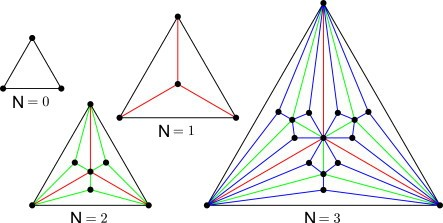
\includegraphics[scale=0.7]{1-s2.0-S0166218X14000195-gr2 (1).jpg}

\medskip

Schéma représentant des ville Apolliniennes avec plusieurs valeurs de $N$.
\end{center}
\end{figureleg}
\medskip
Nous pouvons observer plusieurs propriétés intéressantes de cette ville: 
\begin{itemize}
    \item Le nombre de quartiers auxquels chaque quartier est connecté augmente de manière exponentielle.
    \item Le "diamètre" de la ville, c'est-à-dire le nombre de jours maximal dont le voleur a besoin afin de se déplacer entre deux quartiers quelconques augmente de manière linéaire.
    \item La ville $A_N$ apparaît 3 fois dans la ville $A_{N+1}$.
\end{itemize}

\medskip

A partir de ces propriétés nous conjecturons qu'il existe, en effet, un ville "planaire" telle que Winston ne puisse pas capturer le voleur avec un certain nombre fixe de policiers.

\medskip

Imaginons tout d'abord que Winston puisse capturer le voleur dans $A_N$ avec au minimum $n$ policiers. Nous allons désormais vérifier s' il peut capturer le voleur dans $A_{N+2}$ avec ces $n$ policiers. 

\medskip 

Winston doit savoir si le voleur se trouve dans un tiers de la ville $A_{N+1}$. Pour cela, il doit constamment vérifier les 3 "bornes" de cette sous-ville afin de s'assurer que le voleur ne s'échappe pas. Et lors, de ce fait, il cherche la valeur dans une des 3 sous-sous-villes de cette sous-ville, qui est reliée au maximum à 2 de ces "bornes". Il emploie pour cela les $n$ policiers, mais pour s'assurer que le voleur ne passe pas dans une autre sous-ville, il a besoin d'employer au moins 1 policier de plus.

\medskip

Cette "démonstration" n'était pas forcement très rigoureuse, donc notre conclusion reste une conjecture. Cependant, à partir du paragraphe suivant nous aurions pu conclure qu'il existe une ville planaire telle que Winston ne puisse pas capturer le valeur avec $n$ agents.

\subsection{Conclusion:}

Nous conjecturons qu'en ayant $n$ policiers à disposition, Winston ne peut pas capturer le voleur dans $A_{2n}$. $A_N$ étant toujours une ville planaire, nous conjecturons donc qu'il existe une ville planaire telle que Winston ne puisse pas capturer le voleur avec $n$ policiers pour tout $n$ donné.
\begin{comment}
des exemples de l'an dernier
\begin{figureleg}
\begin{center}
\begin{tikzpicture}[scale=0.5]
% définition des paramètres
\tikzstyle grillemichael=[color=black!30,thin]
\tikzstyle rectmichael=[color=black,very thick]
\tikzstyle echecmichael=[fill=blue!40]
\tikzstyle pointmichael=[color=black,fill=white]
\tikzstyle croixmichael=[color=black,very thick]
\newcommand{\txmin}{1}  % on commence à compter à 1
\newcommand{\txmax}{16} % nombre de villes en largeur
\newcommand{\tymin}{1}
\newcommand{\tymax}{16} % et en hauteur
\newcommand{\rectorigx}{3} % abscisse du point le plus bas
\newcommand{\rectorigy}{5} % ordonnée du point le plus bas
\newcommand{\rectlarg}{4}  % "largeur" du rectangle
\newcommand{\recthaut}{2}  % "hauteur" du rectangle
% la grille
\draw [grillemichael] (\txmin-0.2,\tymin-0.2) grid (\txmax+0.2,\tymax+0.2);
\clip (\txmin-0.2,\tymin-0.2) rectangle (\txmax+0.2,\tymax+0.2);
% l'échiquier !!!! pas automatisé :-(
%\foreach \x in {1,3,...,15}
%\foreach \y in {1,3,...,15}
    %\filldraw[shift={(\x,\y)},echecmichael] (0,0) rectangle (1,1);
%\foreach \x in {2,4,...,14}
%\foreach \y in {2,4,...,14}
    %\filldraw[shift={(\x,\y)},echecmichael] (0,0) rectangle (1,1);
% les points
\foreach \x in {1,3,...,15}
\foreach \y in {1,3,...,15}
    \draw[shift={(\x,\y)},pointmichael] (0,0) circle (0.2);
\foreach \x in {2,4,...,16}
\foreach \y in {2,4,...,16}
    \draw[shift={(\x,\y)},pointmichael] (0,0) circle (0.2);
% les croix
\foreach \x in {1,3,...,15}
\foreach \y in {2,4,...,16}
    \draw[shift={(\x,\y)},croixmichael] (-0.3,-0.3) -- (0.3,0.3) -- (0,0) -- (-0.3,0.3) -- (0.3,-0.3);
\foreach \x in {2,4,...,16}
\foreach \y in {1,3,...,15}
    \draw[shift={(\x,\y)},croixmichael] (-0.3,-0.3) -- (0.3,0.3) -- (0,0) -- (-0.3,0.3) -- (0.3,-0.3);
% le rectangle
\draw [shift={(\rectorigx,\rectorigy)},rectmichael] (0,-0.5)--(-0.5+\rectlarg,-1+\rectlarg)--(\rectlarg-\recthaut,\recthaut+\rectlarg-1.5)--(0.5-\recthaut,-1+\recthaut)--(0,-0.5);
\end{tikzpicture}

\end{center}
\end{figureleg}

 
 

    \medskip
    
    Notons $I_j$ la propriété suivante:
    $$A_{j,n+1}=\dfrac{a_j+2(n-1)}{n}$$
    \begin{itemize}
        \item Initialisation: $$A_{1,n+1}=2(n+1)=\dfrac{4+2(n-1)}{n}=\dfrac{A_{j,2}+2(n-1)}{n}$$
        La propriété $I_n$ est initialisée au rang 1.
        \item Hérédité: Supposons que $I_j$ est vraie pour un certain rang $j$, démontrons que $I_{j+1}$ est vraie:
        $$A_{j+1,n+1}=2(A_{j,n+1}-1)=2\left(\dfrac{a_j+2(n-2)}{n-1}-1\right)$$
        $$2\left(\dfrac{2^j+2+2(n-2)}{n-1}-1\right)=\dfrac{2^{j+1}+4+4(n-2)}{n-1}-2$$
        $$=\dfrac{2^{j+1}+4+4(n-2)-2(n-1)}{n-1}$$
        $$=\dfrac{2^{j+1}+2(n-1)}{n-1}=\dfrac{2^{j+1}+2+2(n-2)}{n-1}$$
        $$=\dfrac{a_{j+1}+2(n-2)}{n-1}$$
        $I_{j+1}$ est vraie, la propriété est donc héréditaire.
        \item Conclusion: La propriété $I_j$ est initialisée au rang 1, la propriété est héréditaire, ainsi $I_j$ est vraie pour tout $J\geq 1$.
    Grace à cette recurrence, nous avons demontre que
    \end{itemize} 
 
 
 
https://www.overleaf.com/project/5cb182ca7bba5b0aeab8f9dd

https://www.overleaf.com/project/5cb183117bba5b0aeab8fa06


 
 \tikzstyle{couleura}=[circle,fill=yellow!90]
    \tikzstyle{couleurb}=[circle,fill=blue!90]
    \tikzstyle{couleurc}=[circle,fill=red!90]
    \tikzstyle{couleurd}=[circle,fill=green!90]
    \tikzstyle{couleure}=[circle,fill=pink!90]
    \tikzstyle{transition}=[rectangle,
    draw=black!50,fill=black!20,thick]
    
\begin{tikzpicture}[x=0.7cm]
        \node at ( 0,0) [couleura] {};
        \draw (0.35,0) -- (0.65,0);
        \node at ( 1,0) [couleurb] {};
        \draw (1.35,0) -- (1.65,0);
        \node at ( 2,0) [couleurc] {};
        \draw[dotted] (2.35,0) -- (3.15,0);
        \node at ( 3.5,0) [couleurd] {};
        \draw [decorate,decoration={brace,mirror,amplitude=3mm},yshift=-3mm](-0.2,0) -- (3.7,0) node[black,midway,yshift=-0.6cm] {\footnotesize $k-1$ demandes};
        
        \draw (3.85,0) -- (4.15,0);
        \node at ( 4.5,0) [couleura] {};
        \draw (4.85,0) -- (5.15,0);
        \node at ( 5.5,0) [couleurb] {};
        \draw (5.85,0) -- (6.15,0);
        \node at ( 6.5,0) [couleurc] {};
        \draw[dotted] (6.85,0) -- (7.65,0);
        \node at ( 8,0) [couleurd] {};
        \draw [decorate,decoration={brace,mirror,amplitude=3mm},yshift=-3mm](4.3,0) -- (8.2,0) node[black,midway,yshift=-0.6cm] {\footnotesize $k-1$ demandes};
        
        \draw[dotted] (8.35,0) -- (11.65,0);
%        \node at ( 8,0) [couleura] {};
%        \draw (8.35,0) -- (8.65,0);
%        \node at ( 9,0) [couleurb] {};
%        \draw (9.35,0) -- (9.65,0);
%        \node at ( 10,0) [couleurc] {};
%        \draw[dotted] (10.35,0) -- (10.65,0);
%        \node at ( 11,0) [couleurd] {};
        \draw [decorate,decoration={brace,mirror,amplitude=3mm},yshift=-13mm](-0.2,0) -- (11.7,0) node[black,midway,yshift=-0.6cm] {\footnotesize $q \cdot (k - 1)$ demandes};
%        \draw (11.35,0) -- (11.65,0);
        \node at ( 12,0) [couleura] {};
        \draw (12.35,0) -- (12.65,0);
        \node at ( 13,0) [couleurb] {};
        \draw (13.35,0) -- (13.65,0);
        \node at ( 14,0) [couleurc] {};
        \draw[dotted] (14.35,0) -- (15.15,0);
        \node at ( 15.5,0) [couleure] {};
        \draw [decorate,decoration={brace,mirror,amplitude=3mm},yshift=-3mm](11.8,0) -- (15.7,0) node[black,midway,yshift=-0.6cm] {\footnotesize $r-1$ demandes};
    \end{tikzpicture}


\begin{figureleg}
\begin{center}
\tikzstyle{memelongueur}=[decoration={markings,
  mark=at position 1/2 with {\draw (0pt,-4pt) -- (0pt,4pt);}},
  postaction={decorate}]
\tikzstyle{mmemelongueur}=[decoration={markings,
  mark=at position .5 with {\draw (-1pt,-4pt) -- (-1pt,4pt);
                            \draw (1pt,-4pt) -- (1pt,4pt);}},
  postaction={decorate}]
\tikzstyle{mmmemelongueur}=[decoration={markings,
  mark=at position 1/2 with {\draw (-2pt,-4pt) -- (-2pt,4pt);
  							\draw (0pt,-4pt) -- (0pt,4pt);
  							\draw (2pt,-4pt) -- (2pt,4pt);}},
  postaction={decorate}]
\definecolor{ududff}{rgb}{0.30196078431372547,0.30196078431372547,1}
\definecolor{ffccww}{rgb}{1,0.8,0.4}


\begin{tikzpicture}[scale=0.5]
% Les axes, graduations, ...
    \tikzstyle grillejulie=[color=blue!20,thin]
\newcommand{\txmin}{0}
\newcommand{\txmax}{20}
\newcommand{\txstep}{1}
\newcommand{\tymin}{-1}
\newcommand{\tymax}{5}
\newcommand{\tystep}{1}
\draw [xstep=\txstep,ystep=\tystep,grillejulie] (\txmin-1.2,\tymin-1.2) grid (\txmax+1.2,\tymax+1.2);
\clip (\txmin-1.2,\tymin-1.2) rectangle (\txmax+1.2,\tymax+1.2);
\draw (-0.2,0) node[below] {\footnotesize O};
% axe des abscisses
\draw [->,thick] (\txmin-1.2,0)--(\txmax+1.2,0);
\foreach \x in {1,...,\txmax}
	\draw[shift={(\x,0)}] (0,0.1) -- (0,-0.1) node[below] {\footnotesize $\x$};
\draw (0.5,5.5) node [anchor=west] {$v_{u_{N(3)}}$};
% axe des ordonnées
\draw [->,thick] (0,\tymin-1.2)--(0,\tymax+1.2);
\foreach \y in {1,...,\tymax} 
	\draw[shift={(0,\y)}] (0.1,0) -- (-0.1,0) node[left] {\footnotesize $\y$};
\draw (20,-1.5) node [anchor=east] {$u_N(3)$ (bleu) et $a_j$ (jaune)};
% Points colorés
\draw [fill=ffccww] (4,0) circle (2.5pt);
\draw [fill=ududff] (5,1) circle (2.5pt);
\draw [fill=ffccww] (6,1) circle (2.5pt);
\draw [fill=ududff] (7,2) circle (2.5pt);
\draw [fill=ududff] (8,2) circle (2.5pt);
\draw [fill=ududff] (9,2) circle (2.5pt);
\draw [fill=ffccww] (10,2) circle (2.5pt);
\draw [fill=ududff] (11,3) circle (2.5pt);
\draw [fill=ududff] (12,3) circle (2.5pt);
\draw [fill=ududff] (13,3) circle (2.5pt);
\draw [fill=ududff] (14,3) circle (2.5pt);
\draw [fill=ududff] (15,3) circle (2.5pt);
\draw [fill=ududff] (16,3) circle (2.5pt);
\draw [fill=ududff] (17,3) circle (2.5pt);
\draw [fill=ffccww] (18,3) circle (2.5pt);
\draw [fill=ududff] (19,4) circle (2.5pt);
\draw [fill=ududff] (20,4) circle (2.5pt);
\draw [fill=ududff] (21,4) circle (2.5pt);
\end{tikzpicture}

\vspace{5mm}
Représentation de la suite $v$ en fonction de $u(3)$ (en bleu) ainsi que de la suite $a$ en fonction de la suite $v$ (en jaune).
\end{center}
\end{figureleg}
\end{comment}
\end{document}
